\documentclass[a4paper]{article}

\def\npart {III}
\def\nterm {Michaelmas}
\def\nyear {2016}
\def\nlecturer {R. Jozsa}
\def\ncourse {Quantum Computation}
\def\nofficial {https://www.qi.damtp.cam.ac.uk/node/261}
\def\nlectures {TT.9}

% Imports
\ifx \nextra \undefined
  \usepackage[pdftex,
    hidelinks,
    pdfauthor={Dexter Chua},
    pdfsubject={Cambridge Maths Notes: Part \npart\ - \ncourse},
    pdftitle={Part \npart\ - \ncourse},
  pdfkeywords={Cambridge Mathematics Maths Math \npart\ \nterm\ \nyear\ \ncourse}]{hyperref}
  \title{Part \npart\ - \ncourse}
\else
  \usepackage[pdftex,
    hidelinks,
    pdfauthor={Dexter Chua},
    pdfsubject={Cambridge Maths Notes: Part \npart\ - \ncourse\ (\nextra)},
    pdftitle={Part \npart\ - \ncourse\ (\nextra)},
  pdfkeywords={Cambridge Mathematics Maths Math \npart\ \nterm\ \nyear\ \ncourse\ \nextra}]{hyperref}

  \title{Part \npart\ - \ncourse \\ {\Large \nextra}}
\fi

\author{Lectured by \nlecturer \\\small Notes taken by Dexter Chua}
\date{\nterm\ \nyear}

\usepackage{alltt}
\usepackage{amsfonts}
\usepackage{amsmath}
\usepackage{amssymb}
\usepackage{amsthm}
\usepackage{booktabs}
\usepackage{caption}
\usepackage{enumitem}
\usepackage{fancyhdr}
\usepackage{graphicx}
\usepackage{mathtools}
\usepackage{microtype}
\usepackage{multirow}
\usepackage{pdflscape}
\usepackage{pgfplots}
\usepackage{siunitx}
\usepackage{tabularx}
\usepackage{tikz}
\usepackage{tkz-euclide}
\usepackage[normalem]{ulem}
\usepackage[all]{xy}

\pgfplotsset{compat=1.12}

\pagestyle{fancyplain}
\lhead{\emph{\nouppercase{\leftmark}}}
\ifx \nextra \undefined
  \rhead{
    \ifnum\thepage=1
    \else
      \npart\ \ncourse
    \fi}
\else
  \rhead{
    \ifnum\thepage=1
    \else
      \npart\ \ncourse\ (\nextra)
    \fi}
\fi
\usetikzlibrary{arrows}
\usetikzlibrary{decorations.markings}
\usetikzlibrary{decorations.pathmorphing}
\usetikzlibrary{positioning}
\usetikzlibrary{fadings}
\usetikzlibrary{intersections}
\usetikzlibrary{cd}

\newcommand*{\Cdot}{\raisebox{-0.25ex}{\scalebox{1.5}{$\cdot$}}}
\newcommand {\pd}[2][ ]{
  \ifx #1 { }
    \frac{\partial}{\partial #2}
  \else
    \frac{\partial^{#1}}{\partial #2^{#1}}
  \fi
}

% Theorems
\theoremstyle{definition}
\newtheorem*{aim}{Aim}
\newtheorem*{axiom}{Axiom}
\newtheorem*{claim}{Claim}
\newtheorem*{cor}{Corollary}
\newtheorem*{defi}{Definition}
\newtheorem*{eg}{Example}
\newtheorem*{fact}{Fact}
\newtheorem*{law}{Law}
\newtheorem*{lemma}{Lemma}
\newtheorem*{notation}{Notation}
\newtheorem*{prop}{Proposition}
\newtheorem*{thm}{Theorem}

\renewcommand{\labelitemi}{--}
\renewcommand{\labelitemii}{$\circ$}
\renewcommand{\labelenumi}{(\roman{*})}

\let\stdsection\section
\renewcommand\section{\newpage\stdsection}

% Strike through
\def\st{\bgroup \ULdepth=-.55ex \ULset}

% Maths symbols
\newcommand{\bra}{\langle}
\newcommand{\ket}{\rangle}

\newcommand{\N}{\mathbb{N}}
\newcommand{\Z}{\mathbb{Z}}
\newcommand{\Q}{\mathbb{Q}}
\renewcommand{\H}{\mathbb{H}}
\newcommand{\R}{\mathbb{R}}
\newcommand{\C}{\mathbb{C}}
\newcommand{\Prob}{\mathbb{P}}
\renewcommand{\P}{\mathbb{P}}
\newcommand{\E}{\mathbb{E}}
\newcommand{\F}{\mathbb{F}}
\newcommand{\cU}{\mathcal{U}}
\newcommand{\RP}{\mathbb{RP}}
\newcommand{\CP}{\mathbb{CP}}

\newcommand{\ph}{\,\cdot\,}

\DeclareMathOperator{\sech}{sech}
\DeclareMathOperator{\cosech}{cosech}
\DeclareMathOperator{\cosec}{cosec}

\DeclareMathOperator{\covol}{covol}
\DeclareMathOperator{\vol}{vol}

\let\Im\relax
\let\Re\relax
\DeclareMathOperator{\Im}{Im}
\DeclareMathOperator{\Re}{Re}
\DeclareMathOperator{\im}{im}
\DeclareMathOperator{\image}{image}
\DeclareMathOperator{\Ann}{Ann}

\DeclareMathOperator*{\res}{res}
\DeclareMathOperator{\Res}{Res}
\DeclareMathOperator{\Ind}{Ind}

\DeclareMathOperator{\tr}{tr}
\DeclareMathOperator{\diag}{diag}
\DeclareMathOperator{\rank}{rank}
\DeclareMathOperator{\card}{card}
\DeclareMathOperator{\spn}{span}
\DeclareMathOperator{\adj}{adj}

\DeclareMathOperator{\erf}{erf}
\DeclareMathOperator{\erfc}{erfc}

\DeclareMathOperator{\ord}{ord}
\DeclareMathOperator{\Sym}{Sym}

\DeclareMathOperator{\sgn}{sgn}
\DeclareMathOperator{\orb}{orb}
\DeclareMathOperator{\stab}{stab}
\DeclareMathOperator{\ccl}{ccl}

\DeclareMathOperator{\lcm}{lcm}
\DeclareMathOperator{\hcf}{hcf}

\DeclareMathOperator{\Int}{Int}
\DeclareMathOperator{\id}{id}

\DeclareMathOperator{\betaD}{beta}
\DeclareMathOperator{\gammaD}{gamma}
\DeclareMathOperator{\Poisson}{Poisson}
\DeclareMathOperator{\binomial}{binomial}
\DeclareMathOperator{\multinomial}{multinomial}
\DeclareMathOperator{\Bernoulli}{Bernoulli}
\DeclareMathOperator{\like}{like}

\DeclareMathOperator{\var}{var}
\DeclareMathOperator{\cov}{cov}
\DeclareMathOperator{\bias}{bias}
\DeclareMathOperator{\mse}{mse}
\DeclareMathOperator{\corr}{corr}

\DeclareMathOperator{\otp}{otp}
\DeclareMathOperator{\dom}{dom}

\DeclareMathOperator{\Root}{Root}
\DeclareMathOperator{\supp}{supp}
\DeclareMathOperator{\rel}{rel}
\DeclareMathOperator{\Hom}{Hom}
\DeclareMathOperator{\Aut}{Aut}
\DeclareMathOperator{\Gal}{Gal}
\DeclareMathOperator{\Mat}{Mat}
\DeclareMathOperator{\End}{End}
\DeclareMathOperator{\Char}{char}
\DeclareMathOperator{\ev}{ev}
\DeclareMathOperator{\St}{St}
\DeclareMathOperator{\Lk}{Lk}
\DeclareMathOperator{\disc}{disc}
\DeclareMathOperator{\Isom}{Isom}
\DeclareMathOperator{\length}{length}
\DeclareMathOperator{\energy}{energy}
\DeclareMathOperator{\area}{area}
\DeclareMathOperator{\Syl}{Syl}
\DeclareMathOperator{\cl}{cl}
\DeclareMathOperator{\fix}{fix}

\newcommand{\GL}{\mathrm{GL}}
\newcommand{\SL}{\mathrm{SL}}
\newcommand{\PGL}{\mathrm{PGL}}
\newcommand{\PSL}{\mathrm{PSL}}
\newcommand{\PSU}{\mathrm{PSU}}
\newcommand{\Or}{\mathrm{O}}
\newcommand{\SO}{\mathrm{SO}}
\newcommand{\U}{\mathrm{U}}
\newcommand{\SU}{\mathrm{SU}}

\renewcommand{\d}{\mathrm{d}}
\newcommand{\D}{\mathrm{D}}

\tikzset{->/.style = {decoration={markings,
                                  mark=at position 1 with {\arrow[scale=2]{latex'}}},
                      postaction={decorate}}}
\tikzset{<-/.style = {decoration={markings,
                                  mark=at position 0 with {\arrowreversed[scale=2]{latex'}}},
                      postaction={decorate}}}
\tikzset{<->/.style = {decoration={markings,
                                   mark=at position 0 with {\arrowreversed[scale=2]{latex'}},
                                   mark=at position 1 with {\arrow[scale=2]{latex'}}},
                       postaction={decorate}}}
\tikzset{->-/.style = {decoration={markings,
                                   mark=at position #1 with {\arrow[scale=2]{latex'}}},
                       postaction={decorate}}}
\tikzset{-<-/.style = {decoration={markings,
                                   mark=at position #1 with {\arrowreversed[scale=2]{latex'}}},
                       postaction={decorate}}}

\tikzset{circ/.style = {fill, circle, inner sep = 0, minimum size = 3}}
\tikzset{mstate/.style={circle, draw, blue, text=black, minimum width=0.7cm}}

\definecolor{mblue}{rgb}{0.2, 0.3, 0.8}
\definecolor{morange}{rgb}{1, 0.5, 0}
\definecolor{mgreen}{rgb}{0.1, 0.4, 0.2}
\definecolor{mred}{rgb}{0.5, 0, 0}

\def\drawcirculararc(#1,#2)(#3,#4)(#5,#6){%
    \pgfmathsetmacro\cA{(#1*#1+#2*#2-#3*#3-#4*#4)/2}%
    \pgfmathsetmacro\cB{(#1*#1+#2*#2-#5*#5-#6*#6)/2}%
    \pgfmathsetmacro\cy{(\cB*(#1-#3)-\cA*(#1-#5))/%
                        ((#2-#6)*(#1-#3)-(#2-#4)*(#1-#5))}%
    \pgfmathsetmacro\cx{(\cA-\cy*(#2-#4))/(#1-#3)}%
    \pgfmathsetmacro\cr{sqrt((#1-\cx)*(#1-\cx)+(#2-\cy)*(#2-\cy))}%
    \pgfmathsetmacro\cA{atan2(#2-\cy,#1-\cx)}%
    \pgfmathsetmacro\cB{atan2(#6-\cy,#5-\cx)}%
    \pgfmathparse{\cB<\cA}%
    \ifnum\pgfmathresult=1
        \pgfmathsetmacro\cB{\cB+360}%
    \fi
    \draw (#1,#2) arc (\cA:\cB:\cr);%
}
\newcommand\getCoord[3]{\newdimen{#1}\newdimen{#2}\pgfextractx{#1}{\pgfpointanchor{#3}{center}}\pgfextracty{#2}{\pgfpointanchor{#3}{center}}}

\def\Xint#1{\mathchoice
   {\XXint\displaystyle\textstyle{#1}}%
   {\XXint\textstyle\scriptstyle{#1}}%
   {\XXint\scriptstyle\scriptscriptstyle{#1}}%
   {\XXint\scriptscriptstyle\scriptscriptstyle{#1}}%
   \!\int}
\def\XXint#1#2#3{{\setbox0=\hbox{$#1{#2#3}{\int}$}
     \vcenter{\hbox{$#2#3$}}\kern-.5\wd0}}
\def\ddashint{\Xint=}
\def\dashint{\Xint-}


\makeatletter
\DeclareRobustCommand{\rvdots}{%
  \vbox{
    \baselineskip4\p@\lineskiplimit\z@
    \kern-\p@
    \hbox{.}\hbox{.}\hbox{.}
  }
}
\newcommand\addstate[3]{
  \pgfmathsetmacro{\y@y}{-#2 * 0.7};
  \pgfmathsetmacro{\x@x}{#3};
  \node [left] at (0, \y@y) {#1};
  \draw (0, \y@y) -- (\x@x, \y@y);
}
\newcommand\addstateend[4]{
  \pgfmathsetmacro{\y@y}{-#2 * 0.7};
  \pgfmathsetmacro{\x@x}{#3};
  \node [left] at (0, \y@y) {#1};
  \node [right] at (\x@x, \y@y) {#4};
  \draw (0, \y@y) -- (\x@x, \y@y);
}

\newcommand\addoperator[3]{
  \node [draw, rectangle, fill=white] at (#3, -#2 * 0.7) {#1};
}
\newcommand\addbigoperator[5]{
  \pgfmathsetmacro{\y@s}{-#2 * 0.7 + 0.2};
  \pgfmathsetmacro{\y@t}{-#3 * 0.7 - 0.2};
  \pgfmathsetmacro{\x@s}{#4};
  \pgfmathsetmacro{\x@t}{#5};
  \pgfmathsetmacro{\x@c}{(\x@s + \x@t)/2};
  \pgfmathsetmacro{\y@c}{(\y@s + \y@t)/2};

  \draw [fill=white] (\x@s, \y@s) rectangle (\x@t, \y@t);
  \node at (\x@c, \y@c) {#1};
}
\newcommand\drawvert[3]{
  \pgfmathsetmacro{\y@y}{-#1 * 0.7};
  \pgfmathsetmacro{\y@yy}{-#2 * 0.7};
  \pgfmathsetmacro{\x@x}{#3};
  \draw (\x@x, \y@y) node [circ] {} -- (\x@x, \y@yy) node [circ] {};
}

\makeatother

\begin{document}
\maketitle
{\small
\setlength{\parindent}{0em}
\setlength{\parskip}{1em}

Quantum mechanical processes can be exploited to provide new modes of information processing that are beyond the capabilities of any classical computer. This leads to remarkable new kinds of algorithms (so-called quantum algorithms) that can offer a dramatically increased efficiency for the execution of some computational tasks. Notable examples include integer factorisation (and consequent efficient breaking of commonly used public key crypto systems) and database searching. In addition to such potential practical benefits, the study of quantum computation has great theoretical interest, combining concepts from computational complexity theory and quantum physics to provide striking fundamental insights into the nature of both disciplines.

The course will cover the following topics:

Notion of qubits, quantum logic gates, circuit model of quantum computation. Basic notions of quantum computational complexity, oracles, query complexity.

The quantum Fourier transform. Exposition of fundamental quantum algorithms including the Deutsch-Jozsa algorithm, Shor's factoring algorithm, Grovers searching algorithm.

A selection from the following further topics (and possibly others):
\begin{enumerate}
  \item Quantum teleportation and the measurement-based model of quantum computation;
  \item Lower bounds on quantum query complexity;
  \item Phase estimation and applications in quantum algorithms;
  \item Quantum simulation for local hamiltonians.
\end{enumerate}

\subsubsection*{Pre-requisites}
It is desirable to have familiarity with the basic formalism of quantum mechanics especially in the simple context of finite dimensional state spaces (state vectors, Dirac notation, composite systems, unitary matrices, Born rule for quantum measurements). Prerequisite notes will be provided on the course webpage giving an account of the necessary material including exercises on the use of notations and relevant calculational techniques of linear algebra. It would be desirable for you to look through this material at (or slightly before) the start of the course. Any encounter with basic ideas of classical theoretical computer science (complexity theory) would be helpful but is not essential.
}
\tableofcontents

\setcounter{section}{-1}
\section{Introduction}
Quantum computation is currently a highly significant and important subject, and is very active in international research.

First of all, it is a fundamental connection between physics and computing. We can think of physics as computing, where in physics, we label states with parameters (ie. numbers), and physical evolution changes these parameters. So we can think of these parameters as encoding information, and physical evolution changes the information. Thus, this evolution can be thought of as a computational process.

More strikingly, we can also view computing as physics! We all have computers, and usually represent information as bits, 0 or 1. We often think of computation as manipulation of these bits, ie. as discrete maths. However, there is no actual discrete bits --- when we build a computer, we need physical devices to represent these bits. When we run a computation on a computer, it has to obey the laws of physics. So we arrive at the idea that the limits of computation are not a part of mathematics, but depend on the laws of physics. Thus, we can associate a ``computing power'' with any theory of physics!

On the other hand, there is also a technology/engineering aspect of quantum computation. Historically, we have been trying to reduce the size of computers. Eventually, we will want to try to achieve miniaturization of computer components to essentially the subatomic scale. The usual boolean operations we base our computations on do not work so well on this small scale, since quantum effects start to kick in. We could try to mitigate these quantum issues and somehow force the bits to act classically, but we can also embrace the quantum effects, and build a quantum computer! There is a lot of recent progress in quantum technology. We are now expecting a 50-qubit quantum computer in full coherent control soon. However, we are not going to talk about implementation in this course.

Finally, apart from the practical problem of building quantum computers, we also have theoretical quantum computer science, where we try to understand how quantum algorithms behave. This is about how we can actually exploit quantum physical facts for computational possibilities beyond classical computers. This will be the focus of the course.

\section{Computational complexity theory}
To appreciate the difference between quantum and classical computing, we need to know how to evaluate an algorithm. This involves understanding some basic complexity theory. But before we could do that, we need to know about computability versus uncomputability.

We will not provide a proper definition of ``computable''. To do so, one comes up with a sensible mathematical model of a computer, and ``computable'' means that theoretical computer can compute it. By the Church-Turing thesis, any two sensible definitions of computability should be equivalent, so we will not spend too much time working out the details.

\begin{eg}
  Let $N$ be an integer. We want to figure out if $N$ a prime. This is clearly computable, since we can try all numbers less than $N$ and see if it divides $N$.
\end{eg}

This is not too surprising, but it turns out there are some problems that are not computable! Most famously, we have the Halting problem.
\begin{eg}[Halting problem]\index{Halting problem}
  Given the code of a computer program, we want to figure out if the computer will eventually halt. In 1936, Turing proved that this problem is uncomputable! So we cannot have a program that determines if an arbitrary program halts!
\end{eg}

For a less arbitrary problem, we have
\begin{eg}
  Given a polynomial with integer coefficients with many variables, eg. $2x^2 y - 17 zw^{19} + x^5 w^3 + 1$, does this have a root in the integers? It was shown in 1976 that this problem is uncomputable as well!
\end{eg}

These results are all for classical computing. If quantum computing is somehow different, can we get around this problems? This turns out not to be the case, for the very reason that all the laws of quantum physics (eg. state descriptions, evolution equations) are all computable on a classical computer (in principle). So it follows that quantum computing, being a quantum process, cannot compute any classical uncomputable problem.

Despite this limitation, quantum computation is still interesting! In practice, there is also the problem of complexity --- the complexity (ie. how hard, how much effort is needed to do the computation) of a quantum computation might be much simpler than the classical counterpart.

To formalize this, we make precise the notion of a computational task.

\begin{defi}[Input string]\index{input string}
  An \emph{input bit string} is a sequence of bits $x = i_1i_2 \cdots i_n$, where each $i_k$ is either $0$ or $1$. We write $B_n$ for the set of all $n$-bit string, and $B = \bigcup_{n \in \N} B_n$. The \emph{input size} is the length $n$. So in particular, if the input is regarded as an actual number, the size is not the number itself, but its logarithm.
\end{defi}

\begin{defi}[Language]
  A \term{language} is a subset $L\subseteq B$.
\end{defi}

\begin{defi}[Decision problem]
  Given a language $L$, the \term{decision problem} is to determine whether an arbitrary $x \in B$ is a member of $L$. The output is thus 1 bit of information, namely yes or no.
\end{defi}
Of course, we can have a more general task with multiple outputs, but for simplicity, we will not consider that case here.

\begin{eg}
  If $L$ is the set of all prime numbers, then the corresponding decision problem is determining whether a number is prime.
\end{eg}

We also have to talk about models of computations. We will only give an intuitive and classical description of it.
\begin{defi}[Computational model]
  A \term{computational model} is a process with discrete steps (elementary computational steps), where each step requires a constant amount of effort/resources to implement.
\end{defi}
If we think about actual computers that works with bits, we can imagine a step as an operation such as ``and'' or ``or''. Note that addition and multiplication are \emph{not} considered a single step --- as the number gets larger, it takes more effort to add or multiply them.

\begin{defi}[Randomized/probabilistic computation]
  This is the same as a usual computational model, but the process also has access to a string $r_1, r_2, r_3, \cdots$ of independent, uniform random bits. In this case, we will often require the answer/output to be correct with ``suitably good'' probability.
\end{defi}

In computer science, there is a separate notion of ``non-deterministic'' computation, which is \emph{different} from probabilistic computation. In probabilistic computation, every time we ask for a random number, we just pick one of the possible output and follows that. With a non-deterministic computer, we simultaneously consider \emph{all} possible paths you can take.

\begin{defi}[Complexity of a computational task (or an algorithm)]
  The \term{complexity} of a computational task or algorithm is the ``consumption of resources as a function of input size $n$''. The resources are usually the time
  \[
    T(n) = \text{number of computational steps needed},
  \]
  and space
  \[
    Sp(n) = \text{number of memory/work space needed}.
  \]
  In each case, we take the worse case input of a given size $n$.
\end{defi}
We usually consider the worst-case scenario, since, eg. for primality testing, there are always some numbers which we can easily rule out as being not prime (eg. even numbers). Sometimes, we will also want to study the average complexity.

In the course, we will mostly focus on the time complexity, and not work with the space complexity itself.

As one would imagine, the actual time or space taken would vary a lot on the actual computational model. Thus, the main question we ask will be whether $T(n)$ grows polynomially or super-polynomially (``exponentially'') with $n$.
\begin{defi}[Polynomial growth]\index{polynomial growth}
  We say $T(n)$ \emph{grows polynomially}, and write
  \[
    T(n) = O(\poly(n)) = O(n^k)
  \]
  for some $k$, if there is some constant $c$, and some integer $k$ and some integer $n_0$ such that $T(n) < c n^k$ for all $n > n_0$.
\end{defi}

The other possible cases are exponential growth, eg. $T(n) = c_1 2^{c_2 n}$, or super-polynomial and sub-exponential growth such as $T(n) = 2^{\sqrt{n}}$ or $n^{\log n}$.

We will usually regard polynomial time processes as ``feasible in practice'', while super-polynomial ones are considered ``infeasible''. Of course, this is not always actually true. For example, we might have a polynomial time of $n^{10^{10^10}}$, or an exponential time of $2^{0.0000\ldots0001 n}$. However, this distinction of polynomial vs non-polynomial is robust, since any computational model can ``simulate'' other computational models in polynomial time. So if something is polynomial in one computational model, it is polynomial in all models.

In general, we can have a more refined complexity classes of decision problems:
\begin{enumerate}
  \item \term{\textbf{P}} (\term{polynomial time}): The class of decision problems having \emph{deterministic} polynomial-time algorithm.
  \item \term{\textbf{BPP}} (\term{bounded error, probabilistic polynomial time}): The class of decision problems having \emph{probabilistic} polynomial time algorithms such that for every input,
    \[
      \mathrm{Prob}(\text{answer is correct}) \geq \frac{2}{3}.
    \]
    The number $\frac{2}{3}$ is sort of arbitrary --- we see that we cannot put $\frac{1}{2}$, or else we can just randomly guess a number. So we need something greater than $\frac{1}{}$, and ``bounded'' refers to it being bounded away from $\frac{1}{2}$. We could replace $\frac{2}{3}$ with any other constant $\frac{1}{2} + \delta$ with $0 < \delta < \frac{1}{2}$, and \textbf{BPP} is the same. This is because if we have a $\frac{1}{2} + \delta$ algorithm, we simply repeat the algorithm $K$ times, and take the majority vote. By the Chernoff bound (a result in probability), the probability that the majority vote is correct is $> 1 - e^{-2 \delta^2 K}$. So as we do more and more runs, the probability of getting a right answer grows exponentially. This can be bigger than an $1 - \varepsilon$ by a suitably large $K$. Since $K$ times a polynomial time is still polynomial time, we still have a polynomial time algorithm.

    These are often considered as ``classically feasible computations'', or ``computable in practice''. In this case, we tolerate small errors, but that is fine in practice, since in genuine computers, random cosmic rays and memory failures can also cause small errors in the result, even for a deterministic algorithm.
\end{enumerate}
It is not known whether \textbf{P} and \textbf{BPP} are the same --- in general, not much is known about whether two complexity classes are the same.

\begin{eg}[Primality testing]
  Let $N$ be an integer. We want to determine if it is prime. The input size is $\log_2 N$. The naive method of primality testing is to test all numbers and see if it divides $N$. We only need to test up to $\sqrt{N}$, since if $N$ has a factor, there must be one below $\sqrt{N}$. The is \emph{not} polynomial time, since we need $\sqrt{N} = 2^{\frac{1}{2} \log N}$ operations, we see that this is exponential time.

  How about a probabilistic algorithm? We can choose a random $k < N$, and see if $k$ divides $N$. This is a probabilistic, polynomial time algorithm, but it is not bounded, since the probability of getting a correct answer is not $> \frac{1}{2}$.

  In reality, primality testing is known to be in \textbf{BPP} (1976), and it is also known to be in \textbf{P} (2004).
\end{eg}

The most famous model for computation is probably a \emph{Turing machine}. However, for our purposes, it is much simpler to work with the \emph{circuit model}.

Classically, for each size $n$, we have a prescribed circuit of Boolean $\AND$, $\OR$ and $\NOT$ gates. We have a \term{circuit family} $\mathcal{C}_1, \mathcal{C}_2, \cdots$, with one for each input size.
% insert diagram

We can think of this as a ``program in machine language''. The computational steps are the gates. The time $T(n)$ is the size of the circuit $\mathcal{C}_n$, ie. the total number of gates in the circuit. A polynomial time computation is one where the size of $\mathcal{C}_n$ grows polynomially in $n$.

We have chosen or primitive gates to be $\AND$, $\OR$ and $\NOT$. It is a fact that this is a \emph{universal set} of gates --- we can make any boolean function $f: B_m \to B_n$ as a circuit of gates from $G$.

Now we go on to quantum stuff!
\section{Quantum computation}
We are again going to introduce our quantum computational model with the circuit model. A single qubit is an element of $\C^2$, with basis vectors
\[
  \bket{0} =
  \begin{pmatrix}
    1 \\ 0
  \end{pmatrix},\quad
  \bket{1} =
  \begin{pmatrix}
    0 \\ 1
  \end{pmatrix}.
\]
For an input $x = i_1i_2\cdots i_n$, we encode this as a qubit $\bket{i_1} \bket{i_2}\cdots\bket{i_n}\bket{0}\cdots\bket{0}$. Now the computational steps are quantum gates, namely unitary operations on designated (few) qubits. For a single qubit, namely an element of $\C^2$, a unitary operation is a $2 \times 2$ matrix. Basic unitary gates commonly used include
\[
  \qX =
  \begin{pmatrix}
    0 & 1\\
    1 & 0
  \end{pmatrix},\quad
  \qZ =
  \begin{pmatrix}
    1 & 0\\
    0 & -1
  \end{pmatrix},\quad
  \qH = \frac{1}{\sqrt{2}}
  \begin{pmatrix}
    1 & 1\\
    1 & -1
  \end{pmatrix},\quad
  \qP_\varphi =
  \begin{pmatrix}1 & 0\\0 & e^{\varphi}\end{pmatrix}
\]
We also have two-qubit gates
\[
  \qCX\bket{i}\bket{j} = \bket{i} X^i\bket{j},\quad CZ
\]
More explicitly, we have
\[
  \qCX =
  \begin{pmatrix}
    1 & 0 & 0 & 0\\
    0 & 1 & 0 & 0\\
    0 & 0 & 0 & 1\\
    0 & 0 & 1 & 0
  \end{pmatrix},\quad
  \qCZ =
  \begin{pmatrix}
    1 & 0 & 0 & 0\\
    0 & 1 & 0 & 0\\
    0 & 0 & 1 & 0\\
    0 & 0 & 0 & -1
  \end{pmatrix},
\]
These will be taken as the basic unitary gates.

After applying a number of these gates, we measure one or more qubit at the end. We also allow intermediate measurements as steps too. These are \emph{not} given by unitary matrices, but in fact these add nothing new (see example sheet 1). This is known as the \term{principle of deferred measurements}. Moreover, we can allow making classical decisions based on the result of the measurement, ie. take different routes depending on what we measure, but again this adds nothing new.

Now what is the analogous notion of a universal set of gates? In the classical case, the set of boolean functions is discrete, and therefore a finite set of gates can be universal. However, in the quantum case, the possible unitary matrices are continuous, so no finite set can be universal.

The idea is to consider approximate universality. We can take the example of the rotations --- there is no single rotation that generates all possible rotations in $\R^2$. However, we can pick a rotation by an irrational angle, and then the set of rotations generated by this rotation is dense in the set of all rotations, and this is good enough.

\begin{defi}[Approximate universality]\index{approximate universality}
  A collection of gates is \emph{approximately universal} if for any unitary matrix $U$, there is some circuit $\tilde{U}$ such that
  \[
    \norm{U - \tilde{U}} < \varepsilon.
  \]
  In other words, we have
  \[
    \sup_{\norm{\psi} = 1} \norm{U\bket{\psi} - \tilde{U} \bket{\psi}} < \varepsilon,
  \]
  where we take the usual norm on the vectors (any two norms are equivalence if the state space is finite dimensional, so it doesn't really matter).
\end{defi}

We will provide some examples without proof.
\begin{eg}
  The infinite set $\{\qCX\} \cup \{\text{all $1$-qubit states}\}$ is exactly universal.
\end{eg}

\begin{eg}
  The collection
  \[
    \{\qH, \qT = \qP_{\pi/4}, \qCX\}
  \]
  is approximately universal.
\end{eg}

\begin{defi}[\textbf{BQP}]\index{\textbf{BQP}}
  The complexity class \textbf{BQP} (bounded error, quantum polynomial time) is the class of all decision problems computable with polynomial quantum circuits with at least $2/3$ probability of being correct.
\end{defi}
We can show that \textbf{BQP} is independent of choice of approximately universal gate set. This is not as trivial as the classical case, since when we switch to a different set, we cannot just replace a gate with an equivalent circuit --- we can only do so approximately, and we have to make sure we control the error appropriately to maintain the bound of $2/3$.

We consider \textbf{BQP} to be the feasible computations with quantum computations.

It is also a fact that \textbf{BPP} is a subset of \textbf{BQP}. This, again, is not a trivial result. Note that in a quantum computation, we act by unitary matrices, which are invertible. However, boolean functions in classical computing are not invertible in general.

However, it turns out that for any classical computation, there is an equivalent computation that uses reversible/invertible boolean gates, with a modest (ie. polynomial) overhead of both space and time resources. Indeed, let $f: B_m \to B_n$ be a boolean function. We consider the function
\begin{align*}
  \tilde{f}: B_{m + n} &\to B_{m + n}\\
  (x, y) &\mapsto (x, y \oplus f(x)),
\end{align*}
where $\oplus$ is the bitwise addition (ie. addition in $(\Z/2\Z)^n$, eg. $011 \oplus 110 = 101$). We call $x$ and $y$ the \term{input register} and \term{output register} respectively.

Now if we set $y = 0$, then we get $f(x)$ in the second component of $\tilde{f}$. So we can easily obtain $f$ from $\tilde{f}$, and vice versa.

\begin{lemma}
  For any boolean function $f: B_m \to B_n$, the function
  \begin{align*}
    \tilde{f}: B_{m + n} &\to B_{m + n}\\
    (x, y) &\mapsto (x, y \oplus f(x)),
  \end{align*}
  is invertible, and in fact an involution, ie. is its own inverse.
\end{lemma}

\begin{proof}
  Simply note that $x \oplus x = 0$ for any $x$, and bitwise addition is associative.
\end{proof}

So we can just consider boolean functions that are invertible. There is an easy way of making this a unitary matrix.
\begin{lemma}
  Let $g: B_k \to B_k$ be a reversible permutation of $k$-bit strings. Then the linear map on $\C^k$ defined by
  \[
    A:\bket{x} \mapsto \bket{g(x)}
  \]
  on $k$ qubits is unitary.
\end{lemma}

\begin{proof}
  This is because the $x$th column of the matrix of $A$ is in fact $A\bket{x} = \bket{g(x)}$, and since $g$ is bijective, the collection of all $\bket{g(x)}$ are all orthonormal.
\end{proof}

Thus, given any $f: B_m \to B_n$, we get the $n + m$-qubit unitary matrix denoted by $U_f$, given by
\[
  U_f\bket{x}\bket{y} = \bket{x}\bket{y \oplus f(x)}.
\]
\subsection{Computation by quantum parallelism}
Suppose we have a function $f: B_m \to B_n$. If we start with $\bket{x}\bket{0\cdots}$, we map
\[
  \begin{tikzcd}
    \bket{x} \bket{0\cdots0} \ar[r, "U_f"] & \bket{x}\bket{f(x)}
  \end{tikzcd}.
\]
So by linearity, we have
\[
  \begin{tikzcd}
    \frac{1}{\sqrt{2^n}}\sum_x \bket{x} \bket{0\cdots0} \ar[r, "U_f"] & \frac{1}{\sqrt{2^n}}\sum_x \bket{x}\bket{f(x)}
  \end{tikzcd}.
\]
We call the final state $\bket{f}$. Now \emph{one} run of $U_f$ gives us the $\bket{f}$ that embodies all exponentially many values of $f(x)$'s. While the state
\[
  \bket{\psi}\frac{1}{\sqrt{2^n}}\sum_x \bket{x}
\]
has exponentially many terms, it can be made in polynomial (and in fact linear) time by $n$ applications of $\qH$, where
\[
  \begin{tikzcd}
    \bket{0} \ar[r, "\qH"] & \frac{1}{\sqrt{2}}(\bket{0} + \bket{1})
  \end{tikzcd}
\]
So for an $n$-qubit state, we have
\[
  \begin{tikzcd}
    \bket{0}\cdots\bket{0} \ar[r, "\qH\otimes \cdots\otimes \qH"] &\frac{1}{\sqrt{2^n}}(\bket{0} + \bket{1})\cdots(\bket{0} + \bket{1})
  \end{tikzcd},
\]
and the result is exactly the starting state we were looking for.

\section{Query complexity}
We are going to come to our first quantum algorithm. Here the input to the computational task is slightly different from what we've got before. Instead of an input $i_1, \cdots, i_n \in B_n$, we have a \emph{black box}/\term{oracle} that computes some $f: B_m \to B_n$. We may have some \emph{a priori} promise on $f$, and we want to determine some property of the function $f$. The only access to $f$ is querying the oracle with its inputs.

The use of $f$ (classical) or $U_f$ (quantum) counts as one step of computation. The \term{query complexity} of this task is the least number of times the oracle needs to be queried. Usually, we do not care much about how many times the other gates are used.

Obviously, if we just query all the values of the function, then we can determine anything about the function, since we have complete information. But we want to see if we can use fewer queries.

\begin{eg}[Balanced vs constant problem]\index{balanced vs constant problem}
  The input black box is a function $f: B_n \to B_1$. The promise is that $f$ is either
  \begin{enumerate}
    \item a \emph{constant} function, ie. $f(x) = 0$ for all $x$, or $f(0) = 1$ for all $x$; or
    \item a \emph{balanced} function, ie. exactly half of its values in $B_n$ are sent to $1$.
  \end{enumerate}
  We want to determine if $f$ is (i) or (ii) with certainty.

  Classically, if we want to find the answer, in the worst case scenario, we will have to perform $2^n/2 + 1$ queries --- if you are really unlucky, you might query a balanced function $2^n/2$ times and get $0$ results.

  Quantumly, we have the \term{Deutsch-Jozsa algorithm}, that answers the question in 1 query!

  A trick we are going to use is something known as ``\term{phase kickback}''. Instead of encoding the result as a single bit, we encode them as $\pm$ signs, ie. as phases of the quantum bits. The ``kickback'' part is about using the fact that we have
  \[
    \bket{a} (e^{i\theta}\bket{b}) = (e^{i\theta}\bket{a})\bket{b},
  \]
  So we might do something to $\bket{b}$ to give it a phase, and then we ``kick back'' the phase on $\bket{a}$, and hopefully obtain something when we measure $\bket{a}$.

  Recall that we have
  \[
    U_f \bket{x}\bket{y} = \bket{x} \bket{y \oplus f(x)}.
  \]
  Here $\bket{x}$ has $n$ qubits, and $\bket{y}$ has 1 qubit.

  The non-obvious thing to do is to set the output register to
  \[
    \bket{\alpha} = \frac{\bket{0} - \bket{1}}{2} = \qH\bket{1} = \qH \qX \bket{0}.
  \]
  We then note that $U_f$ acts by
  \begin{align*}
    \bket{x}\left(\frac{\bket{0} - \bket{1}}{2}\right) &\mapsto \bket{x} \frac{\bket{f(x)} - \bket{1 \oplus f(x)}}{\sqrt{2}}\\
    &=
    \begin{cases}
      \bket{x}\frac{\bket{0} - \bket{1}}{\sqrt{2}}& f(x) = 0\\
      \bket{x}\frac{\bket{1} - \bket{0}}{\sqrt{2}}& f(x) = 1\\
    \end{cases}\\
    &= (-1)^{f(x)}\bket{x}\bket{\alpha}.
  \end{align*}
  Now we do this to the superposition over all possible $x$:
  \[
    \frac{1}{\sqrt{2^n}} \sum \bket{x}\bket{\alpha} \mapsto \left(\frac{1}{\sqrt{2^n}} \sum (-1)^{f(x)}\bket{x}\right) \bket{\alpha}.
  \]
  So one query gives us
  \[
    \bket{\xi_f} = \frac{1}{\sqrt{2^n}} \sum (-1)^{f(x)}\bket{x}.
  \]
  The key observation now is simply that if $f$ is constant, then all the signs are the same. If $x$ is balanced, then exactly half of the signs are $+$ and $-$. The crucial thing is that $\bket{\xi_{f_\text{const}}}$ is orthogonal to $\bket{\xi_{f_\text{balanced}}}$. This is a good thing, since orthogonality is something we can perfectly distinguish with a quantum measurement.

  There is a slight technical problem here. We allow only measurements in the standard $\bket{0}$, $\bket{1}$ basis. So we need want to ``rotate'' our states to the standard basis. Fortunately, recall that
  \[
    \begin{tikzcd}
      \bket{0}\cdots\bket{0} \ar[r, "\qH\otimes \cdots\otimes \qH"] &\frac{1}{\sqrt{2^n}}\sum \bket{x}
    \end{tikzcd},
  \]
  Now recall that $\qH$ is self-inverse, so $H^2 = I$. Thus, if we apply $\qH \otimes\cdots \otimes \qH$ to $\frac{1}{\sqrt{2^n}}\sum \bket{x}$, then we obtain $\bket{0}\cdots\bket{0}$.

  We write
  \[
    \bket{\eta_f} = \qH \otimes \cdots \otimes \qH \bket{\xi_f}.
  \]
  Since $\qH$ is unitary, we still have
  \[
    \bket{\eta_{f_\mathrm{const}}} \perp \bket{\eta_{f_\mathrm{balanced}}}.
  \]
  Now we note that if $f$ is constant, then
  \[
    \eta_{f_\mathrm{const}} = \pm \bket{0}\cdots\bket{0}.
  \]
  If we look at what $\bket{\eta_{f_\mathrm{balanced}}}$ is, it will be a huge mess, but it doesn't really matter --- all that matters is that it is perpendicular to $\bket{0}\cdots\bket{0}$.

  Now when we measure $\eta_f$, if $f$ is a constant function, then we obtain $0\cdots0$ with probability $1$. If it is balanced, then we obtain something that is not $0$ with probability $1$. So we can determine the result with probability $1$.
  \begin{center}
    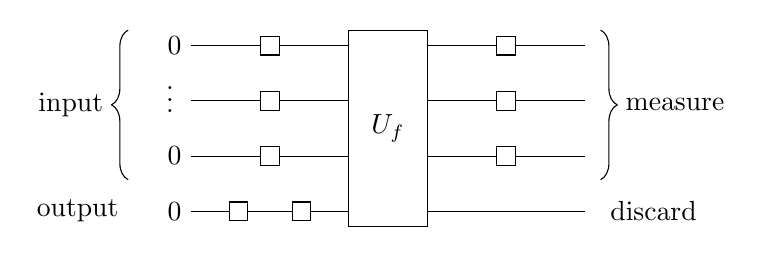
\begin{tikzpicture}
      \addstate{$\bket{0}$}{0}{5};
      \addstate{$\rvdots\;$}{1}{5};
      \addstate{$\bket{0}$}{2}{5};
      \addstate{$\bket{0}$}{3}{5};
      \addoperator{$\qH$}{0}{1};
      \addoperator{$\qH$}{1}{1};
      \addoperator{$\qH$}{2}{1};
      \addoperator{$\qX$}{3}{0.6};
      \addoperator{$\qH$}{3}{1.4};
      \addbigoperator{$U_f$}{0}{3}{2}{3};
      \addoperator{$\qH$}{0}{4};
      \addoperator{$\qH$}{1}{4};
      \addoperator{$\qH$}{2}{4};

      \draw [decorate, decoration={brace, amplitude=6pt}] (-0.8, -1.7) -- (-0.8, 0.2) node [pos=0.5, left] {input\;\;};

      \node [left] at (-0.8, -2.1) {output};

      \draw [decorate, decoration={brace, amplitude=6pt}] (5.2, 0.2) -- (5.2, -1.7) node [pos=0.5, right] {\;\;measure};

      \node [right] at (5.2, -2.1) {discard};
    \end{tikzpicture}
  \end{center}
  This uses exactly one query, with $1 + (n + 1) + n + n = O(n)$ elementary gates.

  Note that for each $a \in B_n$, we can find a special balanced function $f_a$ such that
  \[
    \bket{\eta_{f_a}} = \bket{a}.
  \]
  This is the so-called BV-problem, on the first example sheet. In fact, these are given by
  \[
    f_a(x) = \sum a_i x_i.
  \]
  What if we tolerate error in the balanced vs constant problem? In other words, we only require that the answer is correct with probability $1 - \varepsilon$ with $0 < \varepsilon < \frac{1}{2}$.

  In the quantum case, nothing much changes, since we are probably not going to do better than $1$ query. However, we no longer have a huge benefit over classical algorithms. There is a classical randomized algorithm with $O(\log(1/\varepsilon))$ queries, and in particular does not depend on $n$.

  Indeed, we do it the obvious way --- we choose some $K$ $x$-values uniformly at random from $B_n$, say $x_1, \cdots, x_n$ (where $K$ is fixed and determined later). We then evaluate $f(x_1), \cdots, f(x_n)$.

  If all the outputs are the same, then we say $f$ is constant. If they are not the same, then we say $f$ is balanced.

  If $f$ actually is constant, then the answer is correct with probability $1$. If $f$ is balanced, then each $f(x_i)$ is $0$ or $1$ with equal probability. So the probability of getting the same values for all $x_i$ is
  \[
    \frac{2}{2^K} = 2^{1 - K}.
  \]
  This is our failure probability. So if we pick
  \[
    K > \log_2 (\varepsilon^{-1}) + 1,
  \]
  then we have a failure probability of less than $\varepsilon$.
\end{eg}

Can we decide \emph{every} yes/no question about $f: B_n \to B_1$'s by quantum algorithms with ``a few'' queries? The answer is no. One prominent example is the \term{SAT problem} (\term{satisfiability problem}) --- given $f$, is there an $x$ such that $f(x) = 1$? This is an NP-complete problem. It can be shown that any quantum algorithm (even with a probability $1 - \varepsilon$) needs at least $O(\sqrt{2^n})$, which is achieved by Grover's algorithm. Classically, we need $O(2^n)$ queries, so we have achieved a square root speedup, but not as good as the Deutsch-Jozsa algorithm.

In any case, the Deutsch-Jozsa algorithm demonstrates how we can achieve an exponential benefit with quantum algorithms, but it happens only when we have no error tolerance. In real life scenario, external factors will lead to potential errors anyway, and requiring that we are always correct is not a sensible requirement.

\begin{eg}[Simon's algorithm]\index{Simon's algorithm}
  The \term{Simon's problem} is a promise problem about $f: B_n \to B_n$ with provably exponential separation between claissical ($O(2^{n/4})$) and quantum ($O(n)$) query complexity. The details are on the first example sheet.
\end{eg}

So these are nice examples of benefits of quantum algorithms. However, oracles are rather unnatural problems --- it is rare to just have a black-box access to a function without knowing anything else about the function.

How about more ``normal'' problems? The issue with trying to compare quantum and classical algorithms for ``normal'' problems is that we don't actually have any method to find the lower bound for the computation complexity. For example, while we have not managed to find polynomial prime factorization algorithms, we cannot prove for sure that there isn't any classical algorithm that is polynomial time. However, for the prime factorization problem, we \emph{do} have a quantum algorithm that does much better than all known classical algorithms. This is \emph{Shor's algorithm}, which relies on the toolkit of the quantum Fourier transform.

\section{Quantum Fourier transform and periodicities}

\begin{defi}[Quantum Fourier transform mod $N$]\index{quantum Fourier transform}
  Suppose we have an $N$-dimensional state space with basis $\bket{0}, \bket{1}, \cdots, \bket{N - 1}$ labelled by $\Z/N\Z$. The \emph{quantum Fourier transform mod $N$} is defined by
  \[
    \qQFT: \bket{a} \mapsto \frac{1}{\sqrt{N}} \sum_{b = 0}^{N - 1} e^{2\pi i ab/N} \bket{b}.
  \]
  The matrix entries are
  \[
    [\qQFT]_{ab} = \frac{1}{\sqrt{N}} \omega^{ab},\quad \omega = e^{2\pi i/N},
  \]
  where $a, b = 0, 1, \cdots, N - 1$. We write \term{$\qQFT_n$} for the quantum Fourier transform mod $n$.
\end{defi}
Note that we start counting at $0$, not $1$.

We observe that the matrix $\sqrt{N}\qQFT$ is
\begin{enumerate}
  \item Symmetric
  \item The first (ie. $0$th) row and column are all $1$'s.
  \item Each row and column is a geometric progression $1, r, r^2, \cdots, r^{n - 1}$, where $r = \omega^k$ for the $k$th row or column.
\end{enumerate}

\begin{eg}
  If we look at $\qQFT_2$, then we get our good old $\qH$. However, $\qQFT_4$ is not $H \otimes H$.
\end{eg}

\begin{prop}
  $\qQFT$ is unitary.
\end{prop}

\begin{proof}
  We use the fact that
  \[
    1 + r + \cdots + r^{N - 1} =
    \begin{cases}
      \frac{1 - r^N}{1 - r} & r \not= 1\\
      N & r = 1
    \end{cases}.
  \]
  So if $r = \omega^k$, then we get
  \[
    1 + r + \cdots + r^{N - 1} =
    \begin{cases}
      0 & k \not\equiv 0 \mod N\\
      N & k \equiv 0 \mod N
    \end{cases}.
  \]
  Then we have
  \[
    (\qQFT^\dagger \qQFT)_{ij} = \frac{1}{\sqrt{N}^2} \sum_k \omega^{-ik} \omega^{jk} =\frac{1}{N} \sum_k \omega^{(j-i)k} =
    \begin{cases}
      1 & i = j\\
      0 & i \not= j
    \end{cases}.
  \]
\end{proof}

Now let's consider the periodicity problem.
\begin{eg}\index{Periodicity problem}
  Suppose we are given $f: \Z/N\Z \to Y$. We are promised that $f$ is periodic with some period $r \mid N$, so that
  \[
    f(x + r) = f(x)
  \]
  for all $x$. We also assume that $f$ is injective in each period, so that
  \[
    0 \leq x_1 \not= x_2 \leq r - 1\quad\text{ implies }\quad f(x_1) \not= f(x_2).
  \]
  The problem is to find $r$, with any constant level of error $1 - \varepsilon$ independent of $N$. Since this is not a decision problem, we can allow $\varepsilon > \frac{1}{2}$.

  In the classical setting, if $f$ is viewed as an oracle, then $O(\sqrt{N})$ queries are necessary and sufficient. We are going to show that quantumly, $O(\log \log N)$ queries with $O(\mathrm{poly}(\log N))$ processing steps suffice. In later applications, we will see that the relevant input size is $\log N$, not $N$. So the classical algorithm is exponential time, while the quantum algorithm is polynomial time.

  Note that even if $f$ is given by a simple number-theoretic formula, we still often do not have good classical algorithms to find the period.

  The quantum algorithm is given as follows:
  \begin{enumerate}
    \item Make $\frac{1}{\sqrt{N}} \sum_{x = 0}^{N - 1} \bket{x}$. For example, if $N = 2^n$, then we can make this using $\qH \otimes \cdots \otimes \qH$. If $N$ is not a power of $2$, it is not immediately obvious how we can make this state, but we will discuss this problem later.

    \item We make one query to get
      \[
        \bket{f} = \frac{1}{\sqrt{N}} \sum \bket{x} \bket{f(x)}.
      \]

    \item We now recall that $r \mid N$, Write $N = Ar$, so that $A$ is the number of periods. We measure the second register, and we will see some $y = f(x_0)$ with $x_0$ being the \emph{least} $x$ with $f(x) = y$, ie. it is in the first period. Note that we don't know what $x_0$ is. We just know what $y$ is.

      By periodicity, we know there are exactly $A$ values of $x$ such that $f(x) = y$, namely
      \[
        x_0, x_0 + r, x_0 + 2r, \cdots, x_0 + (A - 1)r.
      \]
      By the Born rule, the first register is collapsed to
      \[
        \bket{\mathrm{per}} = \left(\frac{1}{\sqrt{A}} \sum_{j = 0}^{A - 1} \bket{x_0 + jr}\right) \bket{f(x_0)}.
      \]
      We throw the second register away. Note that $x_0$ is chosen randomly from the first period $0, 1, \cdots, r - 1$.

      What do we do next? If we measure $\bket{\mathrm{per}}$, we obtain a random $j$-value, so what we actually get is a random element ($x_0$th) of a random period ($j$th), namely a uniformly chosen random number in $0, 1, \cdots, N$. This is not too useful.

    \item The solution is the use the quantum Fourier transform, which is not surprising, since Fourier transforms are classically used to extract periodicity information.

      Apply $\qQFT_N$ to $\bket{\mathrm{per})}$ now gives
      \begin{align*}
        \qQFT_N \bket{\mathrm{per}} &= \frac{1}{\sqrt{NA}} \sum_{j = 0}^{n - 1} \sum_{y = 0}^{N - 1} \omega^{(x_0 + jr) y} \bket{y}\\
        &= \frac{1}{\sqrt{NA}} \sum_{y = 0}^{N - 1} \omega^{x_0 y}\left(\sum_{j = 0}^{n - 1}\omega^{jry}\right) \bket{y}
      \end{align*}
      We now see the inner sum is a geometric series. If $\omega^{ry} = 1$, then this sum is just $A$. Otherwise, we have
      \[
        \sum_{j = 0}^{A - 1} \omega^{jry} = \frac{1 - \omega^{rA}}{1 - \omega^{ry}} = \frac{1 - 1}{1 - \omega^{ry}} = 0.
      \]
      So we are left with
      \[
        \qQFT_n \bket{\mathrm{per}} = \sqrt{\frac{A}{N}} \sum_{k = 0}^{r - 1}\omega ^{x_0 k N/r} \bket{k\frac{N}{r}}.
      \]
      Note that before the Fourier transform, the random shift of $x_0$ lied in the label $\bket{x_0 + jr}$. After the Fourier transform, it is not encoded in the phase instead.

    \item Now we can measure the label, and we will some $C$ which is a multiple $k_0 \frac{N}{r}$, where $0 \leq k_0 \leq r - 1$ is chosen uniformly at random. We rewrite this as
      \[
        \frac{k_0}{r} = \frac{C}{N}.
      \]
      We know $C$, because we just measured it, and $N$ is a given in the question. Also, $k_0$ is randomly chosen, and $r$ is what we want. So how do we extract that out?

      If by good chance, we have $k_0$ coprime to $r$, then we can cancel $C/N$ to lowest terms and read off $r$ as the resulting denominator $\tilde{r}$. Note that cancelling $C/N$ to lowest terms can be done quickly by Euclidean algorithm. But how likely are we to be so lucky? We can just find some number theory books, and figure out that the number of natural numbers $< r$ that are coprime to $r$ grows as $O(r/\log \log r)$. More precisely, it is $\sim e^{-\gamma} r/\log \log r$, where $\gamma$ is the other Euler's constant. We note that
      \[
        O\left(\frac{r}{\log \log r}\right) > O\left(\frac{1}{\log \log N}\right).
      \]
      So if $k_0$ is chosen uniformly and randomly, the probability that $k_0$ is coprime to $r$ is at least $O(1/\log \log N)$.

      Note that if $k_0$ is \emph{not} coprime with $r$, then we have $\tilde{r} \mid r$, and in particular $\tilde{r} < r$. So we can check if $\tilde{r}$ is a true period --- we check if $f(0)$ and $f(\tilde{r}$ and see if they are the same. If $\tilde{r}$ is wrong, then they cannot be equal as $f$ is injective in the period.

      While the probability of getting a right answer decreases as $N \to \infty$, we just have to do the experiment many times. From elementary probability, if an event has some (small) success probability $p$, then given any $0 < 1 - \varepsilon < 1$, for $M = - \frac{\log \varepsilon}{p}$ trials, the probability that there is at least one success is $ > 1 - \varepsilon$. So if we repeat the quantum algorithm $O(\log \log N)$ times, and check $\tilde{r}$ each time, then we can get a true $r$ with any constant level of probability.
    \item We can further improve this process --- if we have obtained two attempts $\tilde{r}, \tilde{r}'$, then we know $r$ is at least their least common multiple. So we can in fact achieve this in constant time, if we do a bit more number theory. However, the other parts of the algorithm (eg. cancelling $C/N$ down to lowest terms) still use time polynomial in $\log N$. So we have a polynomial time algorithm.
  \end{enumerate}
\end{eg}

There is one thing we swept under the carpet. We need to find an efficient way of computing the quantum Fourire transform, or else we just hid all our complexity in the quantum Fourier transform.

In general, we would expect that a general unitary operations on $n$ qubits needs $\exp(n)$ elementary circuits. However, the quantum Fourier transform is special.

\begin{fact}
  $\qQFT_{2^n}$ can be implemented by a quantum circuit of size $O(n^2)$.
\end{fact}
The idea of the construction is to mimic the classical fast Fourier transform. An important ingredient of it is:
\begin{fact}
  The state
  \[
    \qQFT_{2^n} \bket{x} = \frac{1}{2^{n/2}} \sum_{y = 0}^{2^n - 1} \omega^{xy}\bket{y}
  \]
  is in fact a product state.
\end{fact}
We can generalize the periodicity problem to arbitrary groups, known as the \emph{hidden subgroup problem}. We are given some oracle for $f: G \to Y$, and we are promised that there is a subgroup $H < G$ such that $f$ is constant and distinct on cosets of $H$ in $G$. We want to find $H$ (we can make ``find'' more precise in two ways --- we can either ask for a set of generators, or provide a way of sampling uniformly from $H$).

In our case, we had $G = (\Z/N\Z, +)$, and $N = Ar$. Our subgroup is then
\[
  H = \{0, r, 2r, \cdots, (A - 1) r\}.
\]
However, we do not know how to efficiently for a group in general.

\subsection{Shor's algorithm}
Given an integer $N$ with $n = \log N$ digits, we will find a factor $1 < K < N$ with constant probability $(1 - \varepsilon)$ in $O(n^3)$ time. The best know classical algorithm is $e^{O(n^{1/3} (\log n)^{2/3})}$.

To do this, we will use the periodicity algorithm. However, there is one subtlety involved. Instead of working in $\Z/n\Z$, to do this algorithm, we need to work in $\Z$. Since computers cannot work with infinitely many numbers, we will have to truncate it somehow.

We now start turning factorization into a periodicity problem. Here are the steps:
Choose a random $1 < a < N$ uniformly randomly, and compute $\hcf(a, N)$. If it is not equal to $1$, then we are finished. Otherwise, by Euler's theorem, there is a least power $r$ of $a$ such that $a^r \equiv 1 \bmod N$. The number $r$ is called the \emph{order} of $a$ mod $N$. It follows that the function $f: \Z \to \Z/N\Z$ given by $f(k) = a^k \bmod N$ has period $r$, and is injective in each period.

Note that $f(k)$ can be efficiently computed in $\poly(\log k)$ time, by repeated squaring. Also note that classically, it is hard to find $r$, even though $f$ has a simple formula!

It was known to Legendre in 1800 that knowing $r$ means we can factor $n$. Suppose we can find $r$, and further suppose $r$ is even. Then we have
\[
  a^r - 1 \equiv (a^{r/2} + 1)(a^{r/2} - 1) \equiv 0 \pmod N.
\]
So $N$ exactly divides the product. By minimality of $r$, we know $N$ does not divide $a^{r/2} - 1$. So if $N$ does not divide $a^{r/2} + 1$ as well, then $\hcf(N, a^{r/2} \pm 1)$ are non-trivial factors of $N$.

For this to work, we needed two assumptions -- $r$ is even, and $a^{r/2} \not\equiv 1 \pmod N$. Fortunately, there is a theorem in number theory that says if $N$ is odd and not a prime power, and $a$ is chosen uniformly at random, then the probability that these two things happen is at least $\frac{1}{2}$. In fact, it is $\geq 1 - \frac{1}{2^{m - 1}}$, where $m$ is the number of prime factors of $N$.

So if we repeat this $k$ times, the probability that they all fail to give a factor is less than $\frac{1}{2^k}$. So this can be as small as we wish.

What about the other possibilities? If $N$ is even, then we would have noticed by looking at the last digit, and we can just write down $2$. If $N = c^\ell$ for $c, \ell > 2$, then there is a classical polynomial time algorithm that outputs $c$, which is a factor.

Everything we've done so far is classical! The quantum part comes in when we want to compute $r$. We know that $f(k) = a^k$ is periodic on $\Z$, which is an infinite domain. So we cannot just apply our periodicity algorithm.

We will work on the domain $D = \{0, 1, \cdots, 2^m - 1\} = \Z/2^m \Z$, where $2^m$ is the least power of $2$ that is $>N^2$. The idea is that we can only have an approximation to what the actual period is. If we pick $2^m$ to be approximately $N$, then it could be that the first $3N/4$ is a single period, and the remaining $N/$ is ``corrupt'' random noise, and it would be difficult to separate out the periodicity information from the corrupt noise. If we take $2^m$ to be at least $N^2$, then we are guaranteed that there will at least be $N$ periods in our data, together with some hopefully minor corruption. Of course, there is no \emph{a priori} reason why we are taking $N^2$ and not, say, $N^3$, but it happens to work.

If $r$ is the true period, then by the division algorithm, there are some $B \geq N$ and $0 \leq b < r$ such that
\[
  2^m = Br + b.
\]
So we have $B$ full periods and one ``corrupt'' one of length $b$.

We now study the effect of corruption on the periodicity algorithm. We again make
\[
  \bket{f} = \frac{1}{\sqrt{2^m}} \sum \bket{x} \bket{f(x)}.
\]
and measure the value of $f$. We then get
\[
  \bket{\mathrm{per}} = \frac{1}{\sqrt{A}} \sum_{k = 0}^{A - 1} \bket{x_0 + kr},
\]
where $A = B$ or $B + 1$, depending on whether $x_0 \leq b$ or not. As before, we apply $\qQFT_{2^m}$ to obtain
\[
  \qQFT_{2^m}\bket{\mathrm{per}} = \sum_{c = 0}^{2^n - 1} \tilde{f}(c) \bket{c}.
\]
When we did this before, with an exact period, most of the $\hat{f}(c)$ is zero. However, this time things are a bit more messy. As before, we have
\[
  \tilde{f}(c) = \frac{\omega^{c x_0}}{\sqrt{A}\sqrt{2^m}} [1 + \alpha + \cdots + \alpha^{A - 1}],\quad \alpha = e^{2\pi i cr/2^m}.
\]
The important question is, when we measure this, which $c$'s will we see with ``good probability''? With exact periodicity, we knew that $\frac{2^m}{r} = A$ is an exact integer. So $\tilde{f}(c) = 0$ except when $c$ is a multiple of $A$. Intuitively, we can think of this as interference, and we had totally destructive and totally constructive interference respectively.

In the inexact case, we will get constructive interference for those $c$ such that the phase $\alpha$ is close to $1$, ie. these are the $c$'s with $\frac{cr}{2^m}$ nearest to integers $k$, and the powers up to $\alpha^{A - 1}$ don't spread too far around the circle. So we avoid cancellations.

So we look at those special $c$'s having this particular property. As $c$ increases from $0$ to $2^m - 1$, the angle $\frac{cr}{2^m}$ increments by $\frac{r}{2^m}$ each time from $0$ up to $r$. So we have $c_k$'s for each $k = 0, 1, \cdots, -r - 1$ such that
\[
  \left|\frac{c_k r}{2^m} - k\right| < \frac{1}{2} \cdot \frac{r}{2^m}.
\]
In other words, we have
\[
  \left|c_k - k\frac{2^m}{r}\right| < \frac{1}{2}.
\]
So the $c_k$ are the integers nearest to the multiples of $2^m/r$.

In $\tilde{f}(c)$, the $\alpha$'s corresponding to the $c_k$'s have the smallest phases, ie. nearest to the positive real axis. We write
\[
  \frac{c_k r}{2^m} = k + \xi,
\]
where
\[
  k \in \Z,\quad |\xi| < \frac{1}{2} \frac{r}{2^m}.
\]
Then we have
\[
  \alpha^n = \exp\left(2\pi i \frac{c_k r}{2^m}n\right) = \exp\left(e\pi i(k + \xi)n\right) = \exp(2 \pi i \xi n)
\]
Now for $n < A$, we know that $|2 \xi n| < \pi$, and thus $1, \alpha, \alpha^2, \cdots, \alpha^{A - 1}$ all lie in the lower half plane or upper half plane.

Doing all the algebra, we find that if $\qQFT\brak{\mathrm{per}}$ is measured, then for any $c_k$ as above, we have
\[
  \mathrm{Prob}(c_k) > \frac{\gamma}{r},
\]
where
\[
  \gamma = \frac{4}{\pi^2} \approx 0.4.
\]
Recall that in the exact periodicity case, the points $c_k$ hit the integers exactly, and instead of $\gamma$ we had $1$. The distribution of the $c$'s then look like:
\begin{center}
  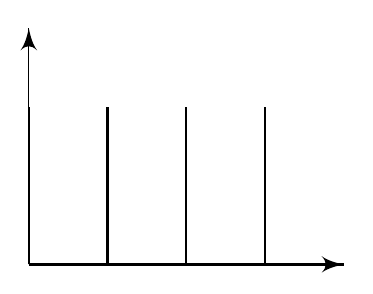
\begin{tikzpicture}
    \draw [->] (0, 0) -- (4, 0);
    \draw [->] (0, 0) -- (0, 3);

    \foreach \x in {0, 1, 2, 3} {
      \draw [thick] (\x, 0) -- (\x, 2);
    }
    \draw [thick] (0, 0) -- (4, 0);
  \end{tikzpicture}
\end{center}
With inexact periods, we obtain something like
\begin{center}
  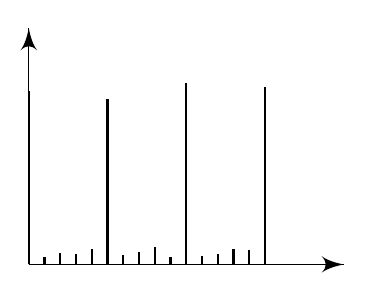
\begin{tikzpicture}
    \draw [->] (0, 0) -- (4, 0);
    \draw [->] (0, 0) -- (0, 3);

    \foreach \x/\y in {0/2.2, 1/2.1, 2/2.3, 3/2.25} {
      \draw [thick] (\x, 0) -- (\x, \y);
    }
    \foreach \x\y in {0.2/0.1,0.4/0.15,0.6/0.13,0.8/0.2,1.2/0.12,1.4/0.16,1.6/0.22,1.8/0.09,2.2/0.11,2.4/0.13,2.6/0.2,2.8/0.18} {
      \draw [thick] (\x, 0) -- (\x, \y);
    }
  \end{tikzpicture}
\end{center}
Now how do we get $r$ from a $c_k$? We know
\[
  \left| \frac{c_k}{2^m} - \frac{k}{r}\right| < \frac{1}{2^{m + 1}} < \frac{1}{2N^2}.
\]
We claim that there is at most 1 fraction $\frac{k}{r}$ with denominator $< N$ such that this inequality holds. So this inequality does uniquely determine $k/r$.

Indeed, suppose $\frac{k}{r}$ and $\frac{k'}{r'}$ both work. Then we have
\[
  \left|\frac{k'}{r'} - \frac{k}{r}\right| = \frac{|k'r - r'k|}{rr'} > \frac{1}{rr'} > \frac{1}{N^2}.
\]
However, we also have
\[
  \left|\frac{k'}{r'} - \frac{k}{r}r\right| \leq \left|\frac{k'}{r'} - \frac{c_k}{2^m}\right| + \left|\frac{c_k}{2^m} - \frac{k}{r}\right| < \frac{1}{2N^2} + \frac{1}{2N^2} = \frac{1}{N^2}.
\]
We introduce the notion of a ``good'' $c_k$ value, which is when $k$ is coprime to $r$. The probability of getting a good $c_k$ is again
\[
  O(1/\log \log r) > O(1/\log \log N).
\]
Note that this is the same rate as the case of exact periodicity, since we have only lost a constant factor of $\gamma$! If we did have such a $c_k$, then now $r$ is uniquely determined.

However, there is still the problem of finding $r$ from a good $c_k$ value. At this point, this is just classical number theory.

We can certainly try all $\frac{k'}{r'}$ with $k' < r' < N$ and find the closets one to $c_k/2^m$, but there are $O(N^2)$ fractions to try, but we want a $O(\mathrm{poly}(\log N))$ algorithm. Indeed, if we were to do it this way, we might as well try all numbers less than $N$ and see if they divide $N$. And this is just $O(N)$!

The answer comes from the nice theory of continued fractions. Any rational number $\frac{s}{t} < 1$ has a continued fraction expansion
\[
  \frac{s}{t} = \cfrac{1}{a_1 + \cfrac{1}{a_2 + \cfrac{1}{a_3 + \cdots}}}.
\]
Indeed to do this, we simply write
\[
  \frac{s}{t} = \cfrac{1}{\cfrac{t}{s}} = \cfrac{1}{a_1 + \cfrac{s_1}{t_1}},
\]
where we divide $t$ by $s$ to get $t = a_1s + s_1$, and then put $t_1 = s$. We then keep going on with $\frac{s_1}{t_1}$. Since the numbers $s_i, t_i$ keep getting smaller, it follows that this process will eventually terminate.

We often write the continued fraction as
\[
  \frac{s}{t} = [a_1, a_2, a_3, \cdots, \cdots, n].
\]
We define the $k$th convergent of $\frac{s}{t}$ to be
\[
  \frac{p_k}{q_k} = [a_1, a_2, \cdots, a_k].
\]
There are some magic results from number theory that gives us a simple recurrence relation for the convergents.
\begin{lemma}
  For $a_1, a_2, \cdots, a_\ell$ any positive reals, we set
  \begin{align*}
    p_0 &= 0 & q_0 &= 1\\
    p_1 &= 1 & q_1 &= a_1
  \end{align*}
  We then define
  \begin{align*}
    p_k &= a_k p_{k - 1} + p_{k - 2}\\
    q_k &= a_k q_{k - 1} + q_{k - 2}
  \end{align*}
  Then we have
  \begin{enumerate}
    \item We have
      \[
        [a_1, \cdots, a_k] = \frac{p_k}{q_k}.
      \]
    \item We also have
      \[
        q_k p_{k - 1} - p_k q_{k - 1} = (-1)^k.
      \]
      In particular, $p_k$ and $q_k$ are coprime.
  \end{enumerate}
\end{lemma}

\begin{thm}
  If $s < t$ are $m$-bit integers, then the continued fraction has length $O(m)$, and all convergents $\frac{p_k}{q_k}$ can be computed in $O(m^3)$ time.
\end{thm}

We can now get to the main useful theorem.
\begin{thm}
  Let $0 < x < 1$ be rational, and suppose $\frac{p}{q}$ is rational with
  \[
    \left|x - \frac{p}{q}\right| < \frac{1}{2q^2}.
  \]
  Then $\frac{p}{q}$ is a convergent of the continued fraction of $x$.
\end{thm}

Then by this theorem, for a good $c$, we know $\frac{k}{r}$ must be a convergent of $\frac{c}{2^m}$. So we compute all convergents find a (unique) one which is within $\frac{1}{2N^2}$ of $\frac{c}{2^m}$. This gives us the value of $r$.

In fact, this last classical part is the slowest part of the algorithm.

\begin{eg}
  Suppose we want to factor $N = 39$. Suppose the random $A$ we chose is $a = 7 < 39$, which is coporime to $N$. Let $r$ be the period of $f(x) = 7^x \bmod 39$.

  We notice
  \[
    1024 = 2^{10} < N^2 = 1621 < 2^{11} = 2048.
  \]
  So we pick $m = 11$. Suppose the measurement of $\qQFT_{2^m}\bket{\mathrm{per}}$ yeilds $c = 853$.

  By the theory, this has a constant probability (approximately $0.4$) to satisfy
  \[
    \left|\frac{853}{2^m} - \frac{k}{r}\right| < \frac{1}{2^{m + 1}} = \frac{1}{2^{12}} < \frac{1}{2N^2}.
  \]
  We also have a probability of $O(1/\log \log r)$ to have $k$ and $r$ coprime. In this case, $c$ is indeed ``good''. So there is a unique $\frac{k}{r}$ satisfying
  \[
    \left|\frac{853}{2048} - \frac{k}{r}\right| < \frac{1}{2^{12}}.
  \]
  So to find $\frac{k}{r}$, we do the continued fraction expansion of $\frac{853}{2048}$. We have
  \[
    \frac{853}{2048} = \cfrac{1}{\cfrac{2048}{853}} = \cfrac{1}{2 + \cfrac{342}{853}} = \cfrac{1}{2 + \cfrac{1}{\cfrac{853}{342}}} = \cfrac{1}{2 + \cfrac{1}{2 + \cfrac{169}{342}}} = \cdots = [2, 2, 2, 42, 4].
  \]
  We can then compute the convergents
  \begin{align*}
    [2] &= \frac{1}{2}\\
    [2, 2] &= \frac{2}{5}\\
    [2, 2, 2] &= \frac{5}{12}\\
    [2, 2, 2, 42] &= \frac{212}{509}\\
    [2, 2, 2, 42, 4] &= \frac{853}{2048}
  \end{align*}
  Of all these numbers, only $\frac{5}{12}$ is within $\frac{1}{2^{12}}$ of $\frac{853}{2048}$ and whose denominator is less than $N = 39$.

  If we do not assume $k$ and $r$ are coprime, then the possible $\frac{k}{r}$ are
  \[
    \frac{5}{12}, \frac{10}{24}, \frac{15}{36}.
  \]
  If we assume that $\frac{k}{r}$ are coprime, then $r = 12$. Indeed, we can try that
  \[
    7^{12} \equiv 1 \pmod {39}.
  \]
  So we now know that
  \[
    39 \mid (7^6 + 1)(7^6 - 1).
  \]
  We now hope/expect with probability $>\frac{1}{2}$ exactly that it goes partly into each factor. We can compute
  \begin{align*}
    7^6 + 1 &= 117650 \equiv 26 \pmod {39}\\
    7^6 - 1 &= 117648 \equiv 24 \pmod {39}
  \end{align*}
  We can then compute
  \[
    \hcf(26, 39) = 13,\quad \hcf(24, 39) = 3 \pmod {39}.
  \]
  We see that $3$ and $13$ are factors of $39$.
\end{eg}

\section{Quantum algorithm for search problems}
Search problems are important in computing. Almost all problems are search problems of some kind.

One important problem is simultaneous constraint satisfaction. For example, when designing a lecture timetable for Part III courses, we need to schedule the courses so that we don't clash two popular courses in the same area, and the courses need to have big enough lecture halls, and you have to make sure a lecturer doesn't have to simultaneously lecture two courses at the same time. This is complicated.

These problems have some common features;
\begin{enumerate}
  \item Given any instance of solution attempt, it is easy to check if it is good or not.
  \item There are exponentially many possible instances to try out.
\end{enumerate}

The fundamental example is the \term{Boolean satisfiability problem} (\term{SAT}). Given a Boolean formula $f: B_n \to B$, we want to know if there is a ``satisfying argument'', ie. if there is an $x$ with $f(x) = 1$.

This has complexity class \textbf{NP}, standing for \emph{non-deterministic polynomial time}. Our definition of \textbf{NP} will involve the notion of a verifier:

\begin{defi}[Verifier]
  We can formulate this as follows: suppose we have a language $L \subseteq B^*$, where
  \[
    B^* = \bigcup_{n \in \N} B_n
  \]
  is the set of all bit strings.

  A \term{verifier} for $L$ is a computation $V(w, c)$ with two inputs $w, c$ such that
  \begin{enumerate}
    \item $V$ halts on all inputs.
    \item If $w \in L$, then for \emph{some} $c$, $V(w, c)$ halts with ``accept''.
    \item If $w \not\in L$, then for \emph{all} $c$, $V(w, c)$ halts with ``reject''.
  \end{enumerate}
  A \term{polynomial time verifier} is a $V$ that runs in polynomial time in $|w|$ (not $|w| + |c|!$).
\end{defi}
We can think of $c$ as ``certificate of membership''. So if you are a member, you can exhibit a certificate of membership that you are in there, and we can check if the certification is valid. However, if you are not a member, you cannot ``fake'' a certificate.

\begin{defi}[Non-deterministic polynomial time problem]\index{\textbf{NP}}\index{non-deterministic polynomial time}
  \textbf{NP} is the class of languages that have polynomial time verifiers.
\end{defi}

\begin{eg}
  The SAT problem is in \textbf{NP}. Here $c$ is the satisfying argument, and $V(f, c)$ just computes $f(c)$ and checks whether it is $1$.
\end{eg}

\begin{eg}
  Determining if a number is composite is in \textbf{NP}, where a certificate is a factor of the number.
\end{eg}
However, it is not immediately obvious that testing if a number is prime is in \textbf{NP}. It is an old result that it indeed is, and recent progress shows that it is in fact in \textbf{P}.

It is rather clear that $\mathbf{P} \subseteq \mathbf{NP}$. Indeed, if we can check membership in polynomial time, then we can also construct a verifier in polynomial time that just throws the certificate away and check directly.

There is another model of \textbf{NP}, via \term{non-deterministic computation}. Recall that in probabilistic computation, in some steps, we had to pick a random number, and picking a different number would lead to a different ``branch''. In the case of non-deterministic computation, we are allowed to take \emph{all} paths at the same time. If \emph{some} of the paths end up being accepting, then we accept the input. If \emph{all} paths reject, then we reject the input.

It is not difficult to see that these definitions of \textbf{NP} are equivalent. Suppose we have a non-deterministic machine that checks if a string is in the language. Then we can construct a verifier whose certificate is a prescription of which particular branch we should follow. Then the verifier just takes the prescription, follows the path described and see if we end up being accepted.

Conversely, if we have a verifier, we can construct a non-deterministic machine by testing a string on \emph{all} possible certificates, and check if any of them accepts.

Unfortunately, we don't know anything about how these different complexity classes compare. We clearly have $\mathbf{P} \subseteq \mathbf{BPP} \subseteq \mathbf{BQP}$ and $\mathbf{P} \subseteq \mathbf{NP}$. However, we do not know if these inclusions are strict, or how $\mathbf{NP}$ compares to the others.

\subsection{Unstructured search problem}
Usually, when we want to search something, the search space we have is structured in some way, and this greatly helps our searching problem. For example, if we have a linearly ordered list of $2^n$, we only need $n$ lookups to find any item with certainty by binary search.

For example, if we have a phone book, then the names are ordered alphabetically. If we want to find someone's phone number, we don't have to look through the whole book. We just open to the middle of the book, and see if the person's name is before or after the names on the page. By one lookup like this, we have already eliminated half of the phone book we have to search through, and we can usually very quickly locate the name.

However, if we know someone's phone number and want to figure out their name, it is pretty much hopeless! This is the problem with unstructured data!

So the problem is as follows: we are given an unstructured database with $N = 2^n$ items and a \emph{unique} good item (or no good items). We can query any item for good or bad-ness. The problem is to find the good item, or determine if one exists.

Classically, $O(N)$ queries are necessary and sufficient. Even if we are asking for a right result with fixed probability $c$, if we pick items randomly to check, then the probability of seeing the ``good'' one in $k$ queries is given by $k/N$. So we still need $O(n)$ queries for any fixed probability.

Quantumly, we have \term{Grover's algorithm}. This needs $O(\sqrt{N}$ queries, and this is both necessary and sufficient.

The database of $N = 2^n$ items will be considered as an oracle $f: B_n \to B_1$. it is promised that there is a unique $x_0 \in B_n$ with $f(x_0) = 1$. The problem is to find $x_0$. Again, we have the quantum oracle
\[
  U_f \bket{x}\bket{y} = \bket{x} \bket{y \otimes f(x)}.
\]
However, we'll use instead $I_{x_0}$ on $n$ qubits given by
\[
  I_{x_0}\bket{x} =
  \begin{cases}
    \bket{x} & x \not= x_0\\
    -\bket{x} & x \not= x_0
  \end{cases}.
\]
This can be constructed from $U_f$ as before, and one use of $I_{x_0}$ can be done with one use of $U_f$.
\begin{center}
  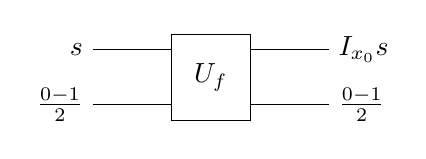
\begin{tikzpicture}
    \addstateend{$\bket{s}$}{0}{3} {$I_{x_0}\bket{s}$};
    \addstateend{$\frac{\bket{0} - \bket{1}}{2}$}{1}{3}{$\frac{\bket{0} - \bket{1}}{2}$};
    \addbigoperator{$U_f$}{0}{1}{1}{2};
  \end{tikzpicture}
\end{center}
We can write $I_{x_0}$ as
\[
  I_{x_0} = I - 2 \bket{x_0} \brak{x_0},
\]
where $I$ is the identity operator.

We are now going to state the \term{Grover's algorithm}, and then later prove that it works.

For convenience, we write
\[
  \qH_n = \underbrace{\qH \otimes \cdots \otimes \qH}_{n\text{ times}}
\]
We start with a uniform superposition
\[
  \bket{\psi_0} = \qH_n \bket{0\cdots0} = \frac{1}{\sqrt{n}} \sum_{\text{all }x} \bket{x}.
\]
We consider the \term{Grover iteration operator} on $n$ qubits given by
\[
  \mathcal{Q} = -\qH_n I_0 \qH_n I_{x_0}.
\]
Here running $I_{x_0}$ requires one query (whereas $I_0$ is ``free'' because it is just $I - 2 \bket{0}\brak{0}$).

Note that all these operators are all real. So we can pretend we are living in the real world and have nice geometric pictures of what is going on. We let $\mathcal{P}(x_0)$ be the (real) plane spanned by $\bket{x_0}$ and $\bket{\psi_0}$. We claim that
\begin{enumerate}
  \item In this plane $\mathcal{P}(x_0)$, this operator $\mathcal{Q}$ is a rotation by $2\alpha$, where
    \[
      \sin\alpha = \frac{1}{\sqrt{N}} = \braket{x_0}{\psi_0}.
    \]
  \item In the orthogonal complement $\mathcal{P}(x_0)^\perp$, we have $\mathcal{Q} = -I$.
\end{enumerate}
We will prove these later on. But if we know this, then we can repeatedly apply $\mathcal{Q}$ to $\bket{\psi_0}$ to rotate it near to $\bket{x_0}$, and then measure. Then we can read on $\bket{x_0}$ with very high probability:
\begin{center}
  \begin{tikzpicture}
    \draw (0, 0) rectangle (5, 5);
    \node at (5, 5) [right] {$\mathcal{P}(x_0)$};
    \draw [->] (1, 1) -- (4, 1) node [right] {$\bket{\psi_0}$};
    \draw [dashed] (1, 1) -- (1, 4);
    \draw [->] (1, 1) -- (2, 4) node [above] {$\bket{x_0}$};

    \draw (1.4, 1) arc(0:71.57:0.4) node [pos=0.5, right] {$\beta$};
    \draw (1, 1.6) arc (90:71.57:0.6) node [pos=0.5, above] {$\alpha$};
  \end{tikzpicture}
\end{center}
The initial angle is
\[
  \cos \beta = \braket{x_0}{\psi_0} = \frac{1}{\sqrt{N}}.
\]
So the number of iterations needed is
\[
  \frac{\cos^{-1}(1/\sqrt{N})}{2 \sin^{-1}(1/\sqrt{N}} = \frac{\beta}{2\alpha}.
\]
In general, this is not an integer, but it will give us $x_0$ with high probability. For large $n$, the number of iterations is approximately
\[
  \frac{\pi/2}{2/\sqrt{N}} = \frac{\pi}{4} \sqrt{N}.
\]
\begin{eg}
  Let's do a boring example with $N = 4$. The initial angle satisfies
  \[
    \cos \beta = \frac{1}{\sqrt{4}} = \frac{1}{2}.
  \]
  So we know
  \[
    \beta = \frac{\pi}{3}.
  \]
  Similarly, we have
  \[
    2\alpha = 2 \sin^{-1}\frac{1}{2} = \frac{\pi}{3}.
  \]
  So $1$ iteration of $\mathcal{Q}$ will rotate $\bket{\psi_0}$ \emph{exactly} to $\bket{x_0}$, so we can find it with \emph{certainty} with 1 lookup.
\end{eg}
Now we prove that this thing actually works. In general, for any unitary $U$ and $I_{\bket{\psi}} = I - 2 \bket{\psi}\brak{\psi}$, we have
\[
  UI_{\bket{\psi}}U^\dagger = UIU^\dagger - 2U \bket{\psi} \brak{\psi} U^\dagger = U_{U \bket{\psi}}.
\]
In particular, since $H_n$ is self-adjoint, ie. $H_n^\dagger H_n$, and that by definition $H_n \bket{0} = \bket{\psi_0}$, we know
\[
  \mathcal{Q} = -H_n I_0 H_n I_{x_0} = I_{\bket{\psi_0}} I_{x_0}.
\]
Next we note that for any $\bket{\psi}$ and $\bket{\xi}$, we know
\[
  I_{\bket{\psi}}\bket{\xi} = \bket{\psi} - 2 \bket{\psi} \braket{\psi}{\xi}.
\]
So this modifies $\bket{\xi}$ by some multiple of $\bket{\psi}$. So we know
\[
  \mathcal{Q}\bket{\psi} = -I_{\bket{\psi_0}} I_{x_0}\bket{\psi}
\]
modifies $\bket{\psi}$ first by some multiple of $\bket{x_0}$, then by some multiple of $\psi_0$. So if $\bket{\xi} \in \mathcal{P}(x_0)$, then $\mathcal{Q} \bket{\psi} \in \mathcal{P}(x_0)$ too! So $\mathcal{Q}$ preserves $\mathcal{P}(x_0)$.

We know that $\mathcal{Q}$ is a unitary, and it is ``real''. So it must be a rotation or a reflection, since these are the only things in $\Or(2)$. We can explicitly figure out what it is. In the plane $\mathcal{P}(x_0)$, we know $I_{\bket{x_0}}$ is reflection in the mirror line perpendicular to $\bket{x_0}$. Similarly, $I_{\bket{\psi_0}}$ is reflection in the mirror line perpendicular to $\bket{\psi_0}$.

We now use the following facts about 2D Euclidean geometry:
\begin{enumerate}
  \item If $R$ is a reflection in mirror $M$ along $\bket{M}$, then $-R$ is reflection in mirror $M^\perp$ along $\bket{M^\perp}$.

    To see this, we know any vector can be written as $a\bket{M} + b \bket{M^\perp}$. Then $R$ sends this to $a \bket{M} - b\bket{M^\perp}$, while $-R$ sends it to $-a \bket{M} + b \bket{M^\perp}$, and this is reflection in $\bket{M^\perp}$.

  \item Suppose we have mirrors $M_1$ and $M_2$ making an angle of $\theta$:
    \begin{center}
      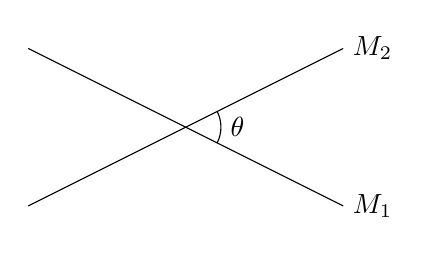
\begin{tikzpicture}
        \draw (-2, 1) -- (2, -1) node [right] {$M_1$};
        \draw (-2, -1) -- (2, 1) node [right] {$M_2$};
        \draw (0.4, -0.2) arc(-26.57:26.57:0.447) node [pos=0.5, right] {$\theta$};
      \end{tikzpicture}
    \end{center}
    Then reflection in $M_1$ then reflection in $M_2$ is the same as rotating counterclockwise by $2\theta$.
\end{enumerate}
So we know
\[
  \mathcal{Q} = -I_{\bket{\psi_0}} I_{\bket{x_0}}
\]
is reflection in $x_0^\perp$ then reflection in $\bket{\psi_0^{\perp\perp}} = \bket{\perp}$. So this is a rotation by $2\alpha$, where $\alpha$ is the angle between $\bket{x_0^\perp}\bket{\psi_0}$, ie.
\[
  \sin \alpha = \cos \beta = \braket{x_0}{\psi_0}.
\]
To prove our second claim that $\mathcal{Q}$ acts as $-\mathbf{1}$ in $\mathcal{P}(x_0)^\perp$, we simply note that if $\bket{\xi} \in \mathcal{P}(x_0)^\perp$, then $\bket{\xi} \perp \bket\psi_0$ and $\xi \perp\bket{x_0}$. So both $I_{\bket{x_0}}$ and $I_{\bket{\psi_0}}$ fix $\bket{\xi}$.

\subsection{Further generalizations}
Suppose we have multiple good items instead, say $r$ of them. We then replace $I_{x_0}$ with $I_f$, where
\[
  I_f \bket{x} =
  \begin{cases}
    -\bket{x} & x\text{ good}\\
    \bket{x} & x\text{ bad}
  \end{cases}
\]
We run the same algorithm as before. We let
\[
  \bket{\psi_{\mathrm{good}}} = \frac{1}{\sqrt{r}} \sum_{x\text{ good}} \bket{x}.
\]
Then now $\mathcal{Q}$ is a rotation through $2\alpha$ with
\[
  \sin \alpha = \braket{\psi_{\mathrm{good}}}{\psi_0} = \sqrt{\frac{r}{N}}.
\]
So for large $N$, we need
\[
  \frac{\pi/2}{2\sqrt{r/N}} = \frac{\pi}{4} \sqrt{\frac{N}{r}},
\]
ie. we have a $\sqrt{r}$ reduction over the unique case.

What if we don't know what $r$ is? The above algorithm would not work, because we will not know when to stop the rotation. However, there are some tricks we can do to fix it.

\subsection{Optimality of Grover's algorithm}
We have the following theorem:
\begin{thm}
  Let $A$ be any quantum algorithm that solves the unique search problem with probability $1 - \varepsilon$ (for any constant $\varepsilon$), with $T$ queries. Then $T$ is at least $O(\sqrt{N})$. In fact, we have
  \[
    T \geq \left(\frac{1}{2} - \varepsilon\right) \sqrt{N}
  \]
  for $\varepsilon < \frac{1}{2}$. In fact, we can prove that
  \[
    T \geq \frac{\pi}{4}(1 - \varepsilon) \sqrt{N}.
  \]
\end{thm}
So Grover's algorithm is not only optimal in the growth rate, but in the constant as well, asymptotically.

Proof is omitted.

\subsection{Amplitude amplification}
Let $G$ be any subspace (``good'' subspace) of the state space $\mathcal{H}$, and $G^\perp$ be its orthogonal complement (``bad'' subspace). Then $\mathcal{H} = G \oplus G^\perp$.

Given any normalized vector $\bket{\psi} \in \mathcal{H}$, we have a unique decomposition with real, non-negative coefficients
\[
  \bket{\psi} = \sin \theta \bket{\psi_g} + \cos \theta \bket{\psi_b}
\]
such that
\[
  \bket{\psi_g} \in G,\quad \bket{\psi_b} \in G^\perp
\]
are normalized.

We introduce reflections that flips $\bket{\psi}$, or any good components, ie.
\[
  I_{\bket{\psi}} = -2\bket{\psi}\brak{\psi},\quad I_g = I - 2P,
\]
where $P$ is the projection onto $G$ given by
\[
  P = \sum_b \bket{b}\brak{b}
\]
for any orthonormal basis $\{\bket{b}\}$ of $G$. This $P$ satisfies
\[
  P \bket{\psi} =
  \begin{cases}
    \bket{\psi} & \bket{\psi} \in G\\
    0 & \bket{\psi} \in G^\perp
  \end{cases}.
\]
We now define the \term{Grover operator}
\[
  \mathcal{Q} = - I_\psi I_G.
\]
\begin{thm}[Amplitude amplification thoerem]\index{amplitude amplification theorem}
  In the $2$-dimensional subspace spanned by $\bket{\psi_g}$ and $\bket{\psi}$ (or equivalently by $\bket{\psi_g}$ and $\bket{\psi_b}$), where
  \[
    \bket{\psi} = \sin \theta \bket{\psi_g} + \cos \theta \bket{\psi_b},
  \]
  we have that $\mathcal{Q}$ is rotation by $2 \theta$.
\end{thm}

\begin{proof}
  We have
  \[
    I_G \bket{\psi_g} = - \bket{\psi_g},\quad I_G \bket{\psi_b} = \bket{\psi_b}.
  \]
  So
  \[
    \mathcal{Q} \bket{\psi_g} = I_\psi \bket{\psi_g}, \quad \mathcal{Q} \bket{\psi_b} = - I_\psi \bket{\psi_b}.
  \]
  We know that
  \[
    I_\psi = I - 2\bket{\psi}\brak{\psi}.
  \]
  So we have
  \begin{align*}
    \mathcal{Q} \bket{\psi_g} &= I_\psi \bket{\psi_g}\\
    &= \bket{\psi_g} - 2(\sin \theta \bket{\psi_g} + \cos \theta \bket{\psi_b})(\sin \theta)\\
    &= (1 - 2 \sin^2 \theta) \bket{\psi_g} - 2 \sin \theta \cos \theta \bket{\psi_b}\\
    &= \cos 2\theta \bket{\psi_g} - \sin 2\theta \bket{\psi_b}\\
    \mathcal{Q} \bket{\psi_b} &= - I_\psi \bket{\psi_b}\\
    &= -\bket{\psi_b} + 2(\sin \theta \bket{\psi_g} + \cos \theta \bket{\psi_b})(\cos \theta)\\
    &= 2 \sin \theta \cos \theta \bket{\psi_g} + (2\cos^2 \theta - 1) \bket{\psi_b}\\
    &= \sin 2 \theta \bket{\psi_g} + \cos 2 \theta \bket{\psi_b}.
  \end{align*}
  So this is rotation by $2 \theta$.

  If we iterate this $n$ times, then we have rotated by $2n \theta$, but we started at $\theta$ from the $\bket{\psi_b}$ direction. So we have
  \[
    \mathcal{Q}^n \bket{\psi} = \sin (2n + 1) \theta \bket{\psi_g} + \cos (2n + 1) \theta \bket{\psi_b}.
  \]
  If we measure $\mathcal{Q}^n\bket{\psi}$ for good versus bad, we know
  \[
    \P(\text{good}) = \sin^2 (2n + 1)\theta,
  \]
  and this is a maximum, when $(2n + 1) \theta = \frac{\pi}{2}$, ie.
  \[
    n = \frac{\pi}{4 \theta} - \frac{1}{2}.
  \]
  For $\theta = \frac{\pi}{b}$ for some integer $b$, then $n$ will be an exact integer. However, for general $\theta$, we know that $n$ is not a n integer. So we use $n$ the nearest integer to $\frac{\pi}{4 \theta} - \frac{1}{2}$, which is approximately
  \[
    \frac{\pi}{4 \theta} = O(\theta^{-1}) = O(1/\sin \theta) = O\left(\frac{1}{\|\text{good projection of }\bket{\psi}\|}\right).
  \]
\end{proof}

\begin{eg}
  Suppose we want to do a Grover search for $r$ good items in $N$ objects. We start with
  \[
    \bket{\psi} = \frac{1}{\sqrt{N}} \sum_{\text{all }x} \bket{x} = \sqrt{\frac{r}{N}}\left(\frac{1}{\sqrt{r}} \sum_{\text{good }x} \bket{x}\right) + \sqrt{\frac{N - r}{N}}\left(\frac{1}{\sqrt{N - r}} \sum_{\text{bad }x} \bket{x}\right).
  \]
  Then $G$ is the subspace spanned by the good $x$'s, and
  \[
    \sin \theta =\sqrt{\frac{r}{N}},
  \]
  So $\mathcal{Q}$ is a rotation by $2\theta$, where
  \[
    \theta = \sin^{-1}\sqrt{\frac{r}{N}} \approx \sqrt{\frac{r}{N}}
  \]
  for $r \ll N$. So we will use $O(\sqrt{r/N})$ operations.
\end{eg}

\begin{eg}
  Let $A$ be any quantum circuit on start state $\bket{0\cdots0}$. Then the final state is $A \bket{0\cdots0}$. The good states are the desired computational outcomes. For example, if $A$ is Shor's algorithm, then the desired outcomes might be the good $c$-values. We can write
  \[
    A\bket{0\cdots0} = a \bket{\psi_g} + b \bket{\psi_b}.
  \]
  The probability of a success in $1$ run is $|a|^2$. So we normally need $O(1/|a|^2)$ repetitions of $A$ to succeed with a given constant probability $1 - \varepsilon$.

  Instead of just measuring the result and hoping for the best, we can use amplitude amplification. We assume we can check if $x$ is good or bad, so we can implement $I_G$. We consider
  \[
    \bket{\psi} = A \bket{0\cdots0}.
  \]
  Then we define
  \[
    \mathcal{Q} = - I_{A\bket{0\cdots0}} I_G = - A I_{\bket{0\cdots0}} A^\dagger I_G.
  \]
  Here we can construct $A^\dagger$ just by reversing the gates in $A$. So all parts are implementable.

  By amplitude amplification, $\mathcal{Q}$ is rotation by $2 \theta$, where $\sin \theta = |a|$. So after
  \[
    n \approx \frac{\pi}{4 \theta} = O(|a|^{-1})
  \]
  repetitions, $A \bket{0\cdots 0}$ will be rotated to very near to $\bket{\psi_g}$, and this will succeed with high probability. This gives us a square root speedup over the naive method.
\end{eg}

\section{Measurement-based quantum computing}
Measurement-based quantum computing is a weird way of doing quantum computation, where instead of using unitary gates, we just keep doing measurements.

\begin{notation}\index{$\bket{\pm_\alpha}$}\index{$\mathcal{B}(\alpha)$}
  We write
  \[
    \bket{\pm_\alpha} = \frac{1}{\sqrt{2}} (\bket{0} \pm e^{-i\alpha} \bket{1}).
  \]
  In particular, we have
  \[
    \bket{\pm_0} = \bket{\pm} = \frac{1}{\sqrt{2}}(\bket{0} \pm \bket{1})
  \]
  Then
  \[
    \mathcal{B}(\alpha) = \{\bket{+_\alpha}, \bket{-_\alpha}\}
  \]
  is an orthonormal basis. We have $1$-qubit gates
  \[
    \qJ(\alpha) = \frac{1}{\sqrt{2}}
    \begin{pmatrix}
      1 & e^{i\alpha}\\
      1 & -e^{i\alpha}
    \end{pmatrix} = H P(\alpha),
  \]
  where
  \[
    \qH = \frac{1}{\sqrt{2}}
    \begin{pmatrix}
      1 & 1\\
      1 & -1
    \end{pmatrix},\quad \qP(\alpha) =
    \begin{pmatrix}
      1 & 0\\
      0 & e^{i\alpha}
    \end{pmatrix}.
  \]
  We also have the ``Pauli gates''
  \[
    \qX=
    \begin{pmatrix}
      0 & 1\\
      1 & 0
    \end{pmatrix},\quad
    \qZ =
    \begin{pmatrix}
      1 & 0\\
      0 & -1
    \end{pmatrix} = \qP(\pi)
  \]
  We also have the 2-qubit gates
  \[
    \qE = \qCZ = \diag(1, 1, 1, -1).
  \]
  We also have $1$-qubit measurements
  \[
    \qM_i(\alpha) = \text{measurement of qubit $i$ in basis $\mathcal{B}(\alpha)$}.
  \]
  The outcome $\bket{+_\alpha}$ is denoted $0$ and the outcome corresponding to $\bket{-_\alpha}$ is denoted $1$.

  We also have $\qM_i(Z)$, which is measurement of qubit $i$ in the standard basis $\{\bket{0}, \bket{1}\}$.

  Suppose we have an undirected graph $G = (V, E)$ with vertices $V$ and edges $E$ with no self-loops and at most one edge between two vertices, we can define the \term{graph state} $\bket{\psi_G}$ that is a state of $|V|$ qubits as follows: for each vertex $i \in V$, introduce a qubit $\bket{+}_i$. For each edge $e: i \to j$, we apply $E_{ij}$ (ie. $E$ operating on the qubits $i$ and $j$). Since all these $E_{ij}$ commute, the order does not matter.

  \begin{eg}
    If $G_1$ is
    \begin{center}
      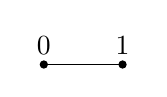
\begin{tikzpicture}
        \node [circ] {};
        \node [above] {$0$};
        \draw (0, 0) -- (1, 0) node [circ] {} node [above] {$1$};
      \end{tikzpicture}
    \end{center}
    then we have
    \[
      \bket{\psi_{G_1}} = E_{12} \bket{+}_1 \bket{+}_2 = \frac{1}{2} [ \bket{00} + \bket{01} + \bket{10} - \bket{11}],
    \]
    and this is an entangled stated.

    If $G_2$ is
    \begin{center}
      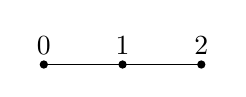
\begin{tikzpicture}
        \node [circ] {};
        \node [above] {$0$};
        \draw (0, 0) -- (1, 0) node [circ] {} node [above] {$1$} -- (2, 0) node [circ] {} node [above] {$2$};
      \end{tikzpicture}
    \end{center}
    then we have
    \[
      \bket{\psi_{G_2}} = E_{12}E_{23} \bket{+}_1 \bket{+}_2 \bket{+}_3.
    \]
  \end{eg}

  A \emph{cluster state} is a graph state $\bket{\psi_G}$ for $G$ being a rectangular $2D$ grid.
  \begin{center}
    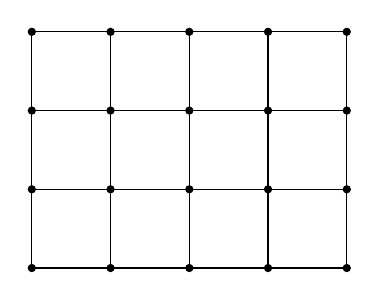
\begin{tikzpicture}
      \draw [step=1cm] (0, 0) grid (4, 3);
      \foreach \x in {0,1,2,3,4} {
        \foreach \y in {0,1,2,3} { \node [circ] at (\x, \y) {}; };
      };
    \end{tikzpicture}
  \end{center}
\end{notation}

\subsection{Main result}
\begin{thm}
  Let $C$ be any quantum circuit on $n$ qubits with a sequence of gates $U_1, \cdots, U_K$ (in order). We have an input state $\bra{\psi_{\mathrm{in}}}$, and we perform $\Z$-measurements on the output states on specified qubits $j = i_1, \cdots, i_k$ to obtain a $k$-bit string.

  We can always simulate the process as follows:
  \begin{enumerate}
    \item Starting resource is a graph state $\bket{\psi_G}$, where $G$ is chosen depending on the connectivity structure of $C$.
    \item The computational steps are $1$-qubit measurements of the form $\qM_i(\alpha)$, ie. measurement in the basis $\mathcal{B}(\alpha)$. This is adaptive --- $\alpha$ may depend on the (random) outcomes $s_1, s_2, \cdots$ of previous measurements.
    \item The computational process is a prescribed (adaptive) sequence $\qM_{i_1}(\alpha_1)$, $\qM_{i_2}(\alpha_2)$, $\cdots$, $\qM_{i_N}(\alpha_N)$, where the qubit labels $i_1, i_2, \cdots, i_N$ all distinct.
    \item To obtain the output of the process, we perform further measurements $\qM(\qZ)$ on $k$ specified qubits not previously measured, and we get results $s_{i_1}, \cdots, s_{i_k}$, and finally the output is obtained by further (simple) \emph{classical} computations on $s_{i_1}, \cdots, s_{i_k}$ as well as the previous $\qM_i(\alpha)$ outcomes.
  \end{enumerate}
\end{thm}
The idea of the last part is that the final measurement $s_{i_1}, \cdots, s_{i_k}$ has to be re-interpret them in light of the $M_i(\alpha_i)$.

This is a funny process, because each measurement $M_i(\alpha)$ is uniformly random, with probability $\frac{1}{2}$ for each outcome, but somehow this is compensated for by the adaptive measurement.

How and why does this work?
\begin{fact}
  The $1$-qubit gates $\qJ(\alpha)$ with $\qE_{i, i\pm 1}$ is a universal set of gate.

  In particular, any $1$-qubit $U$ is a product of $3$ $\qJ$'s.
\end{fact}

We call these $E_{i, i \pm 1}$ \term{nearest neighbour $E_{ij}$'s}.
\begin{proof}
  This is just some boring algebra.
\end{proof}

Note that the restriction that we only have $\qE_{i, i\pm 1}$ is not a really significant restriction, because we can easily implement swaps with them.

So we can assume that our circuit $C$'s gates are all of the form $\qJ(\alpha)$'s or $\qE_{ij}'s$. So it suffices to try to implement these gates in our weird system.

To prove this, we need to prove a lemma, which we will call the $\qJ$-lemma:
\begin{lemma}[$\qJ$-lemma]\index{$\qJ$-lemma}
  For any $1$-qubit state, we have
  \[
    \bket{\psi} = a\bket{0} + b \bket{1}.
  \]
  We consider
  \[
    \qE_{12} (\bket{\psi}_1 \bket{+}_2).
  \]
  Then suppose we measure $\qM_1(\alpha)$. Suppose the outcome is $s_1 \in \{0, 1\}$. Then after measurement, the state of $2$ is
  \[
    \qX^{s_1} \qJ(\alpha) \bket{\psi}.
  \]
  Also, two outcomes $s = 0, 1$ always occurs with probability $\frac{1}{2}$, regardless of the values of $a, b, \alpha$.
\end{lemma}

\begin{proof}
  Just write it out.
\end{proof}

We denote this pictorially as
\begin{center}
  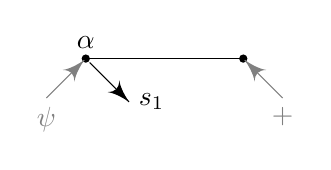
\begin{tikzpicture}
    \node [circ] {};
    \node [above] {$\alpha$};
    \node [circ] at (2, 0) {};
    \draw (0, 0) -- (2, 0);
    \draw [->] (0.05, -0.05) -- +(0.5, -0.5) node [right] {$s_1$};

    \draw [gray, ->] (-0.5, -0.5) node [below] {$\bket{\psi}$} -- (-0.02, -0.02);
    \draw [gray, ->] (2.5, -0.5) node [below] {$\bket{+}$} -- (2.02, -0.02);
  \end{tikzpicture}
\end{center}
If we measure $\qZ$, we denote that by
\begin{center}
  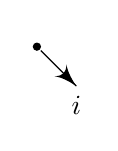
\begin{tikzpicture}
    \node [circ] {};
    \node [above] {$\qZ$};
    \draw [->] (0.05, -0.05) -- (0.5, -0.5) node [below] {$i$};
  \end{tikzpicture}
\end{center}
In fact, we have
\begin{lemma}
  This can be extended if $1$ is just a single qubit part of a larger multi-qubit system $1\mathcal{S}$, ie.
  \[
    \bket{\psi}_{1\mathcal{S}} \bket{\alpha}_\mathcal{S}\bket{0}_1 + \bket{b}_\mathcal{S} \bket{1}.
  \]
  We then apply the $J$-lemma process by adding a new qubit $\bket{+}$ for $2 \not \in \mathcal{S}$, and then query $1$. Then the resulting state is
  \[
    \qX_2^{s_1}\qJ_2(\alpha) \bket{\psi}_{2\mathcal{S}}.
  \]
\end{lemma}
So the $\qJ$-lemma allows us to simulate $\qJ$-gates with measurements. But we want to do many $\qJ$ gates. So we need the concatenation lemma:
\begin{lemma}[Concatenation lemma]
  If we concatenate the process of $\qJ$-lemma on a row of qubits $1, 2, 3, \cdots$ to apply a sequence of $\qJ(\alpha)$ gates, then all the entangling operators $\qE_{12}, \qE_{23}, \cdots$ can be done \emph{first} before any measurements are applied.
\end{lemma}

It is a fact that for any composite quantum system $A \otimes B$, any local actions (unitary gates or measurements) done on $A$ always commutes with anything done on $B$, which is easy to check by expanding out the definition.

\begin{proof}
  For $\bket{\psi}_1 \bket{+}_2 \bket{+}_3\cdots$, we can look at the sequence of $\qJ$-processes in the sequence of operations (left to right):
  \[
    \qE_{12} \qM_1(\alpha_1) \qE_{23}\qM_2(\alpha_2) \qE_{34} \qM_3(\alpha_3)\cdots
  \]
  It is then clear that each $\qE_{ij}$ commutes with all the measurements before it. So we are safe.
\end{proof}

We can now determine the MQC process corresponding to a quantum circuit $C$ of gates $U_1, U_2, \cdots, U_K$ with each $U_i$ either a $\qJ(\alpha)$ or a nearest-neighbour $\qE_{ij}$. We may wlog assume the input state to $C$ is
\[
  \bket{+}\cdots\bket{+}
\]
as any $1$-qubit product state may be written as
\[
  \bket{\psi} = U \bket{+}
\]
for suitable $U$, which is then represented as at most three $\qJ(\alpha)$'s. So we simply prefix $C$ with these $J(\alpha)$ gates.

\begin{eg}
  We can write $\bket{j}$ for $j = 0, 1$ as
  \[
    \bket{j} = \qX^j\qH \bket{+}.
  \]
  We also have
  \[
    \qH = J(0),\quad \qX = \qJ(\pi)\qJ(0).
  \]
\end{eg}

We will write the input qubits as vertical ``blobs'' \begin{tikzpicture}\node [circ] {};\end{tikzpicture}, and all $\qJ(\alpha)$ gates will be implemented by $J$-processes. All nearest-neighbour $\qE_{ij}$'s will just exploit the $\qE$ gates used to make the graph state.

We first do a simple example:
\begin{eg}
  Consider $C$ given by
  \begin{center}
    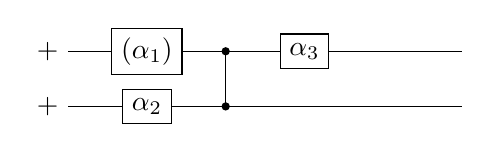
\begin{tikzpicture}
      \addstate{$\bket{+}$}{0}{5};
      \addstate{$\bket{+}$}{1}{5};
      \addoperator{$\qJ(\alpha_1)$}{0}{1};
      \addoperator{$\qJ{\alpha_2}$}{1}{1};
      \addoperator{$\qJ{\alpha_3}$}{0}{3};

      \drawvert{0}{1}{2};
    \end{tikzpicture}
  \end{center}
  and then we measure the outputs $i_1, i_2$ by $\qM(Z)$ measurements.

  We use the graph state
  \begin{center}
    \begin{tikzpicture}
      \node [circ] at (0, 0) {};
      \node [circ] at (1, 0) {};
      \node [circ] at (2, 0) {};
      \node [circ] at (0, -1) {};
      \node [circ] at (1, -1) {};

      \draw (0, 0) -- (2, 0);
      \draw (0, -1) -- (1, -1) -- (1, 0);
    \end{tikzpicture}
  \end{center}
  In other words, we put a node for a $\bket{+}$, horizontal line for a $\qJ(\alpha)$ and a vertical line for an $\qE$.

  If we just measure all the qubits for the $J$-process in the order $\alpha_1, \alpha_2, \alpha_3$:
  \begin{center}
    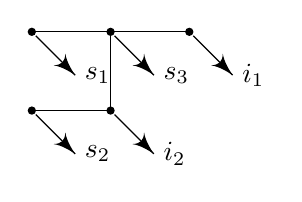
\begin{tikzpicture}
      \node [circ] at (0, 0) {};
      \node [circ] at (1, 0) {};
      \node [circ] at (2, 0) {};
      \node [circ] at (0, -1) {};
      \node [circ] at (1, -1) {};

      \draw (0, 0) -- (2, 0);
      \draw (0, -1) -- (1, -1) -- (1, 0);

      \draw [->] (0.05, -0.05) -- +(0.5, -0.5) node [right] {$s_1$};
      \draw [->] (1.05, -0.05) -- +(0.5, -0.5) node [right] {$s_3$};
      \draw [->] (2.05, -0.05) -- +(0.5, -0.5) node [right] {$i_1$};
      \draw [->] (0.05, -1.05) -- +(0.5, -0.5) node [right] {$s_2$};
      \draw [->] (1.05, -1.05) -- +(0.5, -0.5) node [right] {$i_2$};
    \end{tikzpicture}
  \end{center}
  then we would have effect the circuit
  \begin{center}
    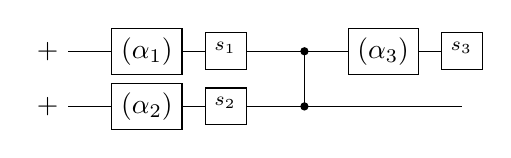
\begin{tikzpicture}
      \addstate{$\bket{+}$}{0}{5};
      \addstate{$\bket{+}$}{1}{5};
      \addoperator{$\qJ(\alpha_1)$}{0}{1};
      \addoperator{$\qJ(\alpha_2)$}{1}{1};

      \addoperator{$\qX^{s_1}$}{0}{2};
      \addoperator{$\qX^{s_2}$}{1}{2};

      \addoperator{$\qJ(\alpha_3)$}{0}{4};
      \addoperator{$\qX^{s_3}$}{0}{5};

      \drawvert{0}{1}{3};
    \end{tikzpicture}
  \end{center}
\end{eg}
Now the problem is to get rid of the $X^i$'s. We know each $X^i$ comes with probability $\frac{1}{2}$. So the probability of them all not appearing is tiny for more complicated circtuis, and we cannot just rely on pure chance for it to turn out right.

To deal with the unwanted $X^i$ ``errors'', we want to commute them out to the end of the circuit. But they do not commute, so we are going to use the following commutation relations:
\[
  J(\alpha) X = e^{i\alpha} Z J(-\alpha)
\]
In other words, up to an overall phase, the following diagrams are equivalent:
\begin{center}
  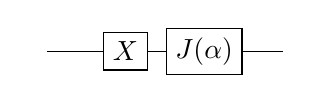
\begin{tikzpicture}
    \addstate{}{0}{3};
    \addoperator{$X$}{0}{1};
    \addoperator{$J(\alpha)$}{0}{2};
  \end{tikzpicture}

  is equivalent to

  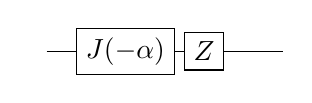
\begin{tikzpicture}
    \addstate{}{0}{3};
    \addoperator{$J(-\alpha)$}{0}{1};
    \addoperator{$Z$}{0}{2};
  \end{tikzpicture}
\end{center}
More generally, we can write
\begin{align*}
  J_i(\alpha) X_i^s &= e^{-i\alpha s} Z_i^s J_i((-1)^s \alpha)\\
  J_i(\alpha) Z_i^s &= X_i^s J_i(\alpha)\\
  E_{ij}Z_i^s = Z_i^s E_{ij}
  E_{ij} X_i^s &= X_i^s Z_i^s E_{ij}
\end{align*}
Here the subscripts tell us which qubit the gates are acting on.

The last one corresponds to
\begin{center}
  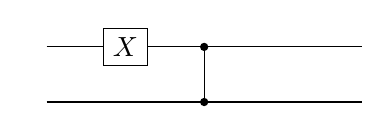
\begin{tikzpicture}
    \addstate{}{0}{4};
    \addstate{}{1}{4};
    \addoperator{$X$}{0}{1};
    \drawvert{0}{1}{2}
  \end{tikzpicture}
  is equivalent to
  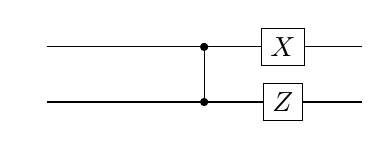
\begin{tikzpicture}
    \addstate{}{0}{4};
    \addstate{}{1}{4};
    \drawvert{0}{1}{2}
    \addoperator{$X$}{0}{3};
    \addoperator{$Z$}{1}{3};
  \end{tikzpicture}
\end{center}
All of these are good, except for the first one where we have a funny phase and the angle is negatived. The phase change is irrelevant because it doesn't affect measurements, but the sign changes are problematic. To fix this, we need to use adaptive measurements.

\begin{eg}
  Consider the simpler $1$-qubit circuit
  \begin{center}
    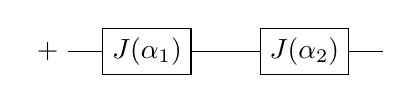
\begin{tikzpicture}
      \addstate{$\bket{+}$}{0}{4};
      \addoperator{$J(\alpha_1)$}{0}{1};
      \addoperator{$J(\alpha_2)$}{0}{3};
    \end{tikzpicture}
  \end{center}
  We first prepare the graph sate
  \begin{center}
    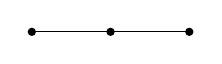
\begin{tikzpicture}
      \node [circ] at (0, 0) {};
      \node [circ] at (1, 0) {};
      \node [circ] at (2, 0) {};

      \draw (0, 0) -- (2, 0);
    \end{tikzpicture}
  \end{center}
  We now measure the first qubit to get
  \begin{center}
    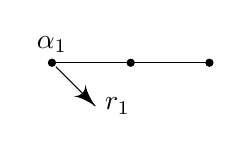
\begin{tikzpicture}
      \node [circ] at (0, 0) {};
      \node [circ] at (1, 0) {};
      \node [circ] at (2, 0) {};

      \draw (0, 0) node [above] {$\alpha_1$} -- (2, 0);
      \draw [->] (0.05, -0.05) -- +(0.5, -0.5) node [right] {$r_1$};
    \end{tikzpicture}
  \end{center}
  We have thus done
  \begin{center}
    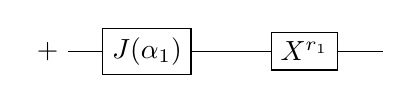
\begin{tikzpicture}
      \addstate{$\bket{+}$}{0}{4};
      \addoperator{$J(\alpha_1)$}{0}{1};
      \addoperator{$X^{r_1}$}{0}{3};
    \end{tikzpicture}
  \end{center}
  To deal with the unwanted $X^{r_1}$, we note that
  \begin{center}
    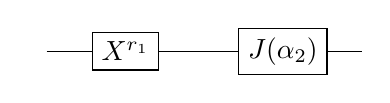
\begin{tikzpicture}
      \addstate{}{0}{4};
      \addoperator{$X^{r_1}$}{0}{1};
      \addoperator{$J(\alpha_2)$}{0}{3};
    \end{tikzpicture}
    is equivalent to
    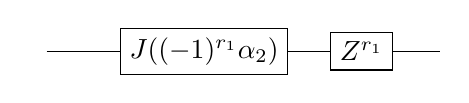
\begin{tikzpicture}
      \addstate{}{0}{5};
      \addoperator{$J((-1)^{r_1}\alpha_2)$}{0}{2};
      \addoperator{$Z^{r_1}$}{0}{4};
    \end{tikzpicture}
  \end{center}
  So we adapt the sign of the second measurement angle to depend on the previous measurement result:
  \begin{center}
    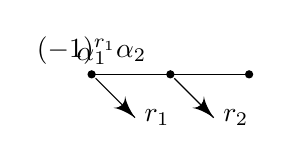
\begin{tikzpicture}
      \node [circ] at (0, 0) {};
      \node [circ] at (1, 0) {};
      \node [circ] at (2, 0) {};

      \draw (0, 0) -- (2, 0);
      \node [above] at (0, 0) {$\alpha_1$};
      \node [above] at (0, 0) {$(-1)^{r_1}\alpha_2$};
      \draw [->] (0.05, -0.05) -- +(0.5, -0.5) node [right] {$r_1$};
      \draw [->] (1.05, -0.05) -- +(0.5, -0.5) node [right] {$r_2$};
    \end{tikzpicture}
  \end{center}
  Then this measurement results in
  \begin{center}
    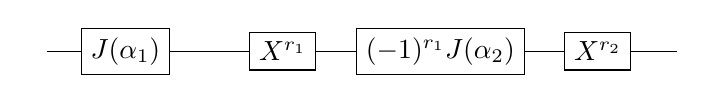
\begin{tikzpicture}
      \addstate{}{0}{8};
      \addoperator{$J(\alpha_1)$}{0}{1};
      \addoperator{$X^{r_1}$}{0}{3};
      \addoperator{$(-1)^{r_1}J(\alpha_2)$}{0}{5};
      \addoperator{$X^{r_2}$}{0}{7};
    \end{tikzpicture}

    is equivalent to

    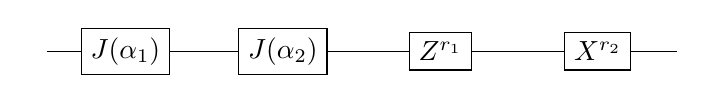
\begin{tikzpicture}
      \addstate{}{0}{8};
      \addoperator{$J(\alpha_1)$}{0}{1};
      \addoperator{$J(\alpha_2)$}{0}{3};
      \addoperator{$Z^{r_1}$}{0}{5};
      \addoperator{$X^{r_2}$}{0}{7};
    \end{tikzpicture}
  \end{center}
  If we had further $J$-gates, we need to commute both $Z^{r_1}$ and $X^{r_2}$ over.

  Note that while we are introducing a lot of funny $X$'s and $Z$'s, these are all we've got, and the order of applying them does not matter, as they anti-commute:
  \[
    XZ = -ZX.
  \]
  So if we don't care about the phase, they effectively commute.

  Also, since $X^2 = Z^2 I$, we only need to count the number of $X$'s and $Z$'s mod 2, which is very helpful.

  Now what do we do with the $Z$ and $X$ at the end? For the final $Z$-measurement, having moved everything to the end, we simply reinterpret the final, actual $Z$-measurement result $j$:
  \begin{enumerate}
    \item The $Z$-gate does not affect outcome or probability of a $Z$-measurement, becasuse if
      \[
        \bket{\psi} = a \bket{0} + b \bket{1},
      \]
      then
      \[
        Z \bket{\psi} = a \bket{0} - b \bket{1}.
      \]
      So the probabilities of $\bket{0}$ and $\bket{1}$ are $|a|^2$ and $|b|^2$ regardless.

    \item The $X$ gate simply interchanges the labels, while leavining probabilities the same, because if
      \[
        \bket{\psi} = a \bket{0} + b \bket{1},
      \]
      then
      \[
        X \bket{\psi} = a \bket{1} + b \bket{0}.
      \]
  \end{enumerate}
  So we ignore all $Z$-errors, and for each $X^r$ error, we just modify the seen measurement outcome $j$ by $j \mapsto j \oplus r$.
\end{eg}

\subsubsection*{Logical depth of a measurement pattern}
Measurements can always be done ``left to right'', implementing the gates in order. However, we don't have to do that. Recall that quantum operations on disjoint qubits always commute. So the $M_i(\alpha)$ measurements can be performed simultaneously if the angles $\alpha$ do not depend on other measurements. This gives us a novel way to parallel a computation.

For example, in our simple example, we can start by first measuring $r_1$ and $j$, and then measuring $r_2$ after we know $r_1$. In particular, we can \emph{first} measure the ``answer'' $j$, before we do any other thing! The remaining measurements just tell us how we should interpret the answer.

In general, we can divide the measurements into ``layers'' --- the first layer consists of all measurements that do not require any adaptation. The second layer then consists of the measurements that only depends on the first layer.

The \term{logical depth} is then the least number of layers needed.

\section{Phase estimation algorithm}
Given a unitary operator $U$ and an eigenstate $\bket{v_\varphi}$ such that
\[
  U \bket{V_\varphi} = 2^{2\pi i \varphi} \bket{v_\varphi}
\]
with $0 \leq \varphi < 1$, we want to estimate $\varphi$ to $n$ binary bits of precision:
\[
  \varphi \approx 0.i_1 i_2 i_3 \cdots i_n = \frac{i_1}{2} + \frac{i_2}{2^2} + \cdots + \frac{i_n}{2^n}.
\]
We will need a $c-U^k$ for integers $k$ such that
\begin{align*}
  \qcd U^k\bket{0}\bket{\xi} &= \bket{0}\bket{\xi}\\
  \qcd U^k\bket{1}\bket{\xi} &= \bket{1} U^k\bket\xi,
\end{align*}
where $\bket{0}, \bket{1}$ are 1-qubit states, and $\bket{\xi}$ is a general $d$-dimensional register.

Note that we have
\[
  U^k \bket{v_\varphi} = e^{2\pi i k \varphi}\bket{v_\varphi},
\]
and we have
\[
  \qcd U^k = (\qcd U)^k,
\]
Note that if we are given $U$ as a formula or a circuit \emph{description}, then we can readily implement $\qcd U$ by adding control to each gate. However, if $U$ is a quantum black-box, then we need further info. For example, it suffices to have an eigenstate $\bket{\alpha}$ with \emph{known} eigenvalue $e^{i\alpha}$. However, we will not bother ourselves with that, and just assume that we can indeed implement it.

In fact, we will use a ``generalized'' controlled $U$ given by
\[
  \bket{x} \bket{\xi} \mapsto \bket{x}U^x \bket{\xi},
\]
where $\bket{x}$ has $n$ qubits with $x \in \Z_n$. We will make this from $\qcd U^k = (\qcd U)^k$ as follows: for % check if Z_n or Z_{2^n}
\[
  x = x_{n - 1} \cdots x_1 x_0 = x_0 + 2^1 x_1 + 2^2 x_2 + \cdots + 2^{n - 1}x_{n - 1},
\]
we write $\qcd U^k_i$ for the controlled $U^k$ controlled by $i$. Then we just construct
\[
  U^{2^0}_0 U^{2^1}_1 \cdots U^{2^{n - 1}}_{n - 1}.
\]
Now if input $\bket{\xi} = \bket{v_{\varphi}}$, then we get
\[
  2^{\pi i \varphi x} \bket{x} \bket{v_\varphi}.
\]
To do phase estimation, we superpose the above over all $x = 0, 1, 2, \cdots, 2^{n - 1}$ and use $\bket{\xi} = \bket{v_\varphi}$. So we construct our starting state by
\[
  \bket{s} = \qH \otimes \cdots \otimes \qH \bket{0\cdots0} = \frac{1}{\sqrt{2^n}} \sum_{\text{all }x} \bket{x}.
\]
Now if we apply the generalized control $U$, we obtain
\[
  \underbrace{\left(\frac{1}{\sqrt{2^n}} \sum_x e^{2\pi i \varphi x}\bket{x}\right)}_{\bket{A}} \bket{v_\psi}.
\]
Finally, we apply the inverse Fourier transform $\qQFT_{2^n}^{-1}$ to $\bket{A}$ and measure to see $y_0, y_1, \cdots, y_{n -1 }$ on lines $0, 1, \cdots, n - 1$. Then we simply output
\[
  0.y_0 y_1 \cdots y_{n - 1} = \frac{y_0}{2} + \frac{y_1}{4} + \cdots + \frac{y_{n - 1}}{2^n} = \frac{y_0 y_1 \cdots y_{n - 1}}{2^n}.
\]
as the estimate of $\varphi$.

Why does this work? Suppose $\varphi$ actually only had $n$ binary digits. Then we have
\[
  \varphi = 0.z_0 z_1 \cdots \cdots z_{n - 1} = \frac{z}{2^n},
\]
where $z \in \Z_{2^n}$. Then we have
\[
  \bket{A} = \frac{1}{\sqrt{2^n}} \sum_x 2^{2\pi i x z/2^n} \bket{x},
\]
which is the Fourier transform of $\bket{z}$. So the inverse Fourier transform of $\bket{A}$ is exactly $\bket{Z}$ and we get $\varphi$ exactly with certainty.

If $\varphi$ has more than $n$ bits, say
\[
  \varphi = 0.z_0z_1 \cdots z_{n - 1}z_n z_{n + 1} \cdots,
\]
then we have
\begin{thm}
  If the measurements in the above algorithm give $y_0, y_1, \cdots, y_n$ and we output
  \[
    \theta = 0.y_0 y_1 \cdots y_{n - 1},
  \]
  then
  \begin{enumerate}
    \item The probability that $\theta$ is $\varphi$ to $n$ digits is at least $\frac{4}{\pi^2}$.
    \item The probability that $|\theta - \varphi| \geq \varepsilon$ is at most $O(1/(2^n \varepsilon))$.
  \end{enumerate}
\end{thm}
The proofs are rather boring and easy algebra.

So for any fixed desired accuracy $\varepsilon$, the probability to fail to get $\varphi$ to this accuracy falls \emph{exponentially} with $n$.

Note that if $\qcd U^{2^k}$ is implemented as $(\qcd U)^{2^k}$, then the algorithm would need
\[
  1 + 2 + 4 + \cdots + 2^{n - 1} = 2^{n - 1}
\]
many $\qcd U$ gates. But for some special $U$'s, this $\qcd U^{2^k}$ can be implemented in polynomial time in $k$.

For example, in Kitaer's factor algorithm, for $\hcf(a, N) = 1$, we use
\[
  U: \bket{m} \mapsto \bket{am \bmod N}
\]
Then we have
\[
  U^{2^k}\bket{m} = \bket{a^{2^k}m},
\]
which we can implement by repeated squaring.

Now what if we didn't have an eigenstate to being with? If instead of $\bket{v_\varphi}$, we used a general input state $\bket{\xi}$, then we can write
\[
  \bket{\xi} = \sum_j c_j \bket{v_{\varphi_j}},
\]
where
\[
  U \bket{v_{\varphi_j}} = e^{2\pi i \varphi_j}\bket{v_{\varphi_j}}.
\]
Then in the phase estimation algorithm, just before the final measurement, we have managed to get ourselves
\[
  \bket{0\cdots0}\bket{\xi} \to \sum_j c_j \bket{\varphi_j} \bket{v_{\varphi_j}}.
\]
Then when we measure some \emph{one} of the $\varphi_j$'s (or an approximation of it) with probability $|c_j|^2$. Note that this is \emph{not} some average of them. Of course, we don't know which one we got, but we still get some meaningful.

\subsubsection*{Quantum counting}
An application of this is the quantum counting problem. Given $f: B_n \to B$ with $k$ good $x$'s, we want to estimate the number $k$.

Recall the Grove iteration operator $\mathcal{Q}_G$ is rotation through $2\theta$ in a $2$-dimensional plane spanned by
\[
  \bket{\psi_0} = \frac{1}{\sqrt{2^n}} \sum_x \bket{x}
\]
and its good projection, and $\theta$ is given by
\[
  \sin \theta \approx \theta = \sqrt{\frac{k}{N}}.
\]
Now the eigenvalues of this rotation in the plane are
\[
  e^{2i \theta}, e^{-2i\theta}.
\]
So either eigenvalue will suffice to get $k$.

We will equivalently write
\[
  e^{i2\theta} = e^{2\pi i \varphi}
\]
with
\[
  0 \leq \varphi < 1.
\]
Then $\pm 2 \theta$ is equivalent to $\varphi$ or $1 - \varphi$, where $\varphi$ is small.

Now we don't have an eigenstate, but we can start with any state in the plane, $\bket{\psi_0}$. We then do phase estimation with it. We will then get either $\varphi$ or $1 - \varphi$ with some probabilities, but we don't mind which one we get, since we can obtain one from the other, and we can tell them apart because $\varphi$ is small.


\printindex
\end{document}
